\documentclass[fleqn,10pt]{SelfArx}

\usepackage[spanish]{babel}
\usepackage{float}

\setlength{\columnsep}{0.55cm}
\setlength{\fboxrule}{0.75pt}

\definecolor{color1}{RGB}{0,0,90}
\definecolor{color2}{RGB}{0,20,20}

\usepackage{hyperref}

\hypersetup{
	hidelinks,
	colorlinks,
	breaklinks=true,
	urlcolor=color2,
	citecolor=color1,
	linkcolor=color1,
	bookmarksopen=false,
	pdftitle={Examen Parcial No.1 - Sistemas Inteligentes},
	pdfauthor={Alioth Polo},
}

%----------------------------------------------------------------------------------------

\JournalInfo{ITSE -- Inteligencia Artificial, D-IA-3\_1, 3er Cuatrimestre}
\Archive{Examen Parcial No.1 -- Sistemas Inteligentes}

\PaperTitle{Examen Parcial No.1: Redes Neuronales Aplicadas a Problemas de Ingenier\'ia}

\Authors{Alioth Polo\textsuperscript{1} -- C\'edula: 8-1034-398}
\affiliation{\textsuperscript{1}\textit{Estudiante de Inteligencia Artificial, D-IA-3\_1, ITSE}}
\affiliation{\textbf{Profesor}: Dr. Sergio Enrique Pinto}

\Keywords{Redes Neuronales --- TensorFlow --- Keras --- Gemelo Digital --- Proyectiles --- Aproximaci\'on de Funciones}
\newcommand{\keywordname}{Palabras Clave}

%----------------------------------------------------------------------------------------

\Abstract{En este trabajo se presentan las soluciones al Examen Parcial No.1 del curso de Sistemas Inteligentes. Se desarrollaron cuatro problemas utilizando redes neuronales artificiales implementadas con TensorFlow y Keras: (1) modelado de curvas de descarga de bater\'ia a diferentes temperaturas, (2) aproximaci\'on de pares de curvas y determinaci\'on de puntos de intersecci\'on, (3) simulaci\'on del choque de dos proyectiles mediante an\'alisis f\'isico y redes neuronales, y (4) construcci\'on de un gemelo digital de un sensor de presi\'on. Los resultados demuestran la capacidad de las redes neuronales tipo MLP para aproximar funciones con alta precisi\'on.}

\renewcommand{\abstractname}{Resumen}

%----------------------------------------------------------------------------------------

\begin{document}

\maketitle

\tableofcontents

\thispagestyle{empty}

%----------------------------------------------------------------------------------------

\section*{Introducci\'on}
\addcontentsline{toc}{section}{Introducci\'on}

Las redes neuronales artificiales han demostrado ser herramientas poderosas para la aproximaci\'on de funciones, el modelado de sistemas f\'isicos y la creaci\'on de gemelos digitales \cite{goodfellow2016}. Su capacidad como aproximadores universales, demostrada por Hornik et al. \cite{hornik1989}, permite representar relaciones complejas entre variables a partir de datos de entrenamiento.

En el presente examen parcial se aplican redes neuronales tipo Perceptr\'on Multicapa (MLP), implementadas con TensorFlow \cite{tensorflow2015} y Keras \cite{keras2015}, para resolver cuatro problemas de ingenier\'ia: descarga de bater\'ias, intersecci\'on de curvas, colisi\'on de proyectiles y modelado de sensores de presi\'on. En todos los casos se utiliza el optimizador Adam \cite{kingma2014} y la funci\'on de p\'erdida MSE (Error Cuadr\'atico Medio).

%----------------------------------------------------------------------------------------

\section{Problema 1: Descarga de Bater\'ia (20 Puntos)}

Se desarrollaron redes neuronales para modelar la curva de descarga de voltaje de una bater\'ia en funci\'on del per\'iodo de descarga, a cuatro temperaturas distintas: 25\textdegree C, 10\textdegree C, 0\textdegree C y $-$10\textdegree C.

\subsection{Datos}

Se dispone de 11 puntos de medici\'on para cada temperatura, con el tiempo de descarga variando de 0 a 20 minutos. La Tabla~\ref{tab:bateria} muestra los datos utilizados.

\begin{table}[H]
	\caption{Datos de voltaje de descarga (V) por temperatura}
	\centering
	\small
	\begin{tabular}{ccccc}
		\toprule
		t (min) & 25\textdegree C & 10\textdegree C & 0\textdegree C & $-$10\textdegree C \\
		\midrule
		0  & 4.20 & 3.75 & 3.50 & 3.20 \\
		2  & 4.05 & 3.70 & 3.55 & 3.30 \\
		4  & 3.95 & 3.68 & 3.58 & 3.38 \\
		6  & 3.88 & 3.65 & 3.59 & 3.42 \\
		8  & 3.82 & 3.62 & 3.58 & 3.40 \\
		10 & 3.77 & 3.58 & 3.55 & 3.35 \\
		12 & 3.72 & 3.54 & 3.50 & 3.30 \\
		14 & 3.68 & 3.50 & 3.45 & 3.25 \\
		16 & 3.63 & 3.45 & 3.38 & 3.20 \\
		18 & 3.57 & 3.38 & 3.30 & 3.12 \\
		20 & 3.40 & 3.25 & 3.15 & 3.00 \\
		\bottomrule
	\end{tabular}
	\label{tab:bateria}
\end{table}

\subsection{Arquitectura de la Red}

Para cada temperatura se entren\'o una red neuronal independiente con la siguiente arquitectura:

\begin{itemize}[noitemsep]
	\item Capa de entrada: 1 neurona (tiempo normalizado)
	\item Capa oculta 1: 10 neuronas, activaci\'on ReLU
	\item Capa oculta 2: 10 neuronas, activaci\'on ReLU
	\item Capa de salida: 1 neurona, activaci\'on lineal
\end{itemize}

Se utiliz\'o el optimizador Adam con tasa de aprendizaje 0.01, funci\'on de p\'erdida MSE, 2000 \'epocas m\'aximas y parada temprana con paciencia de 200 \'epocas.

\subsection{Resultados}

\begin{figure*}[ht]\centering
	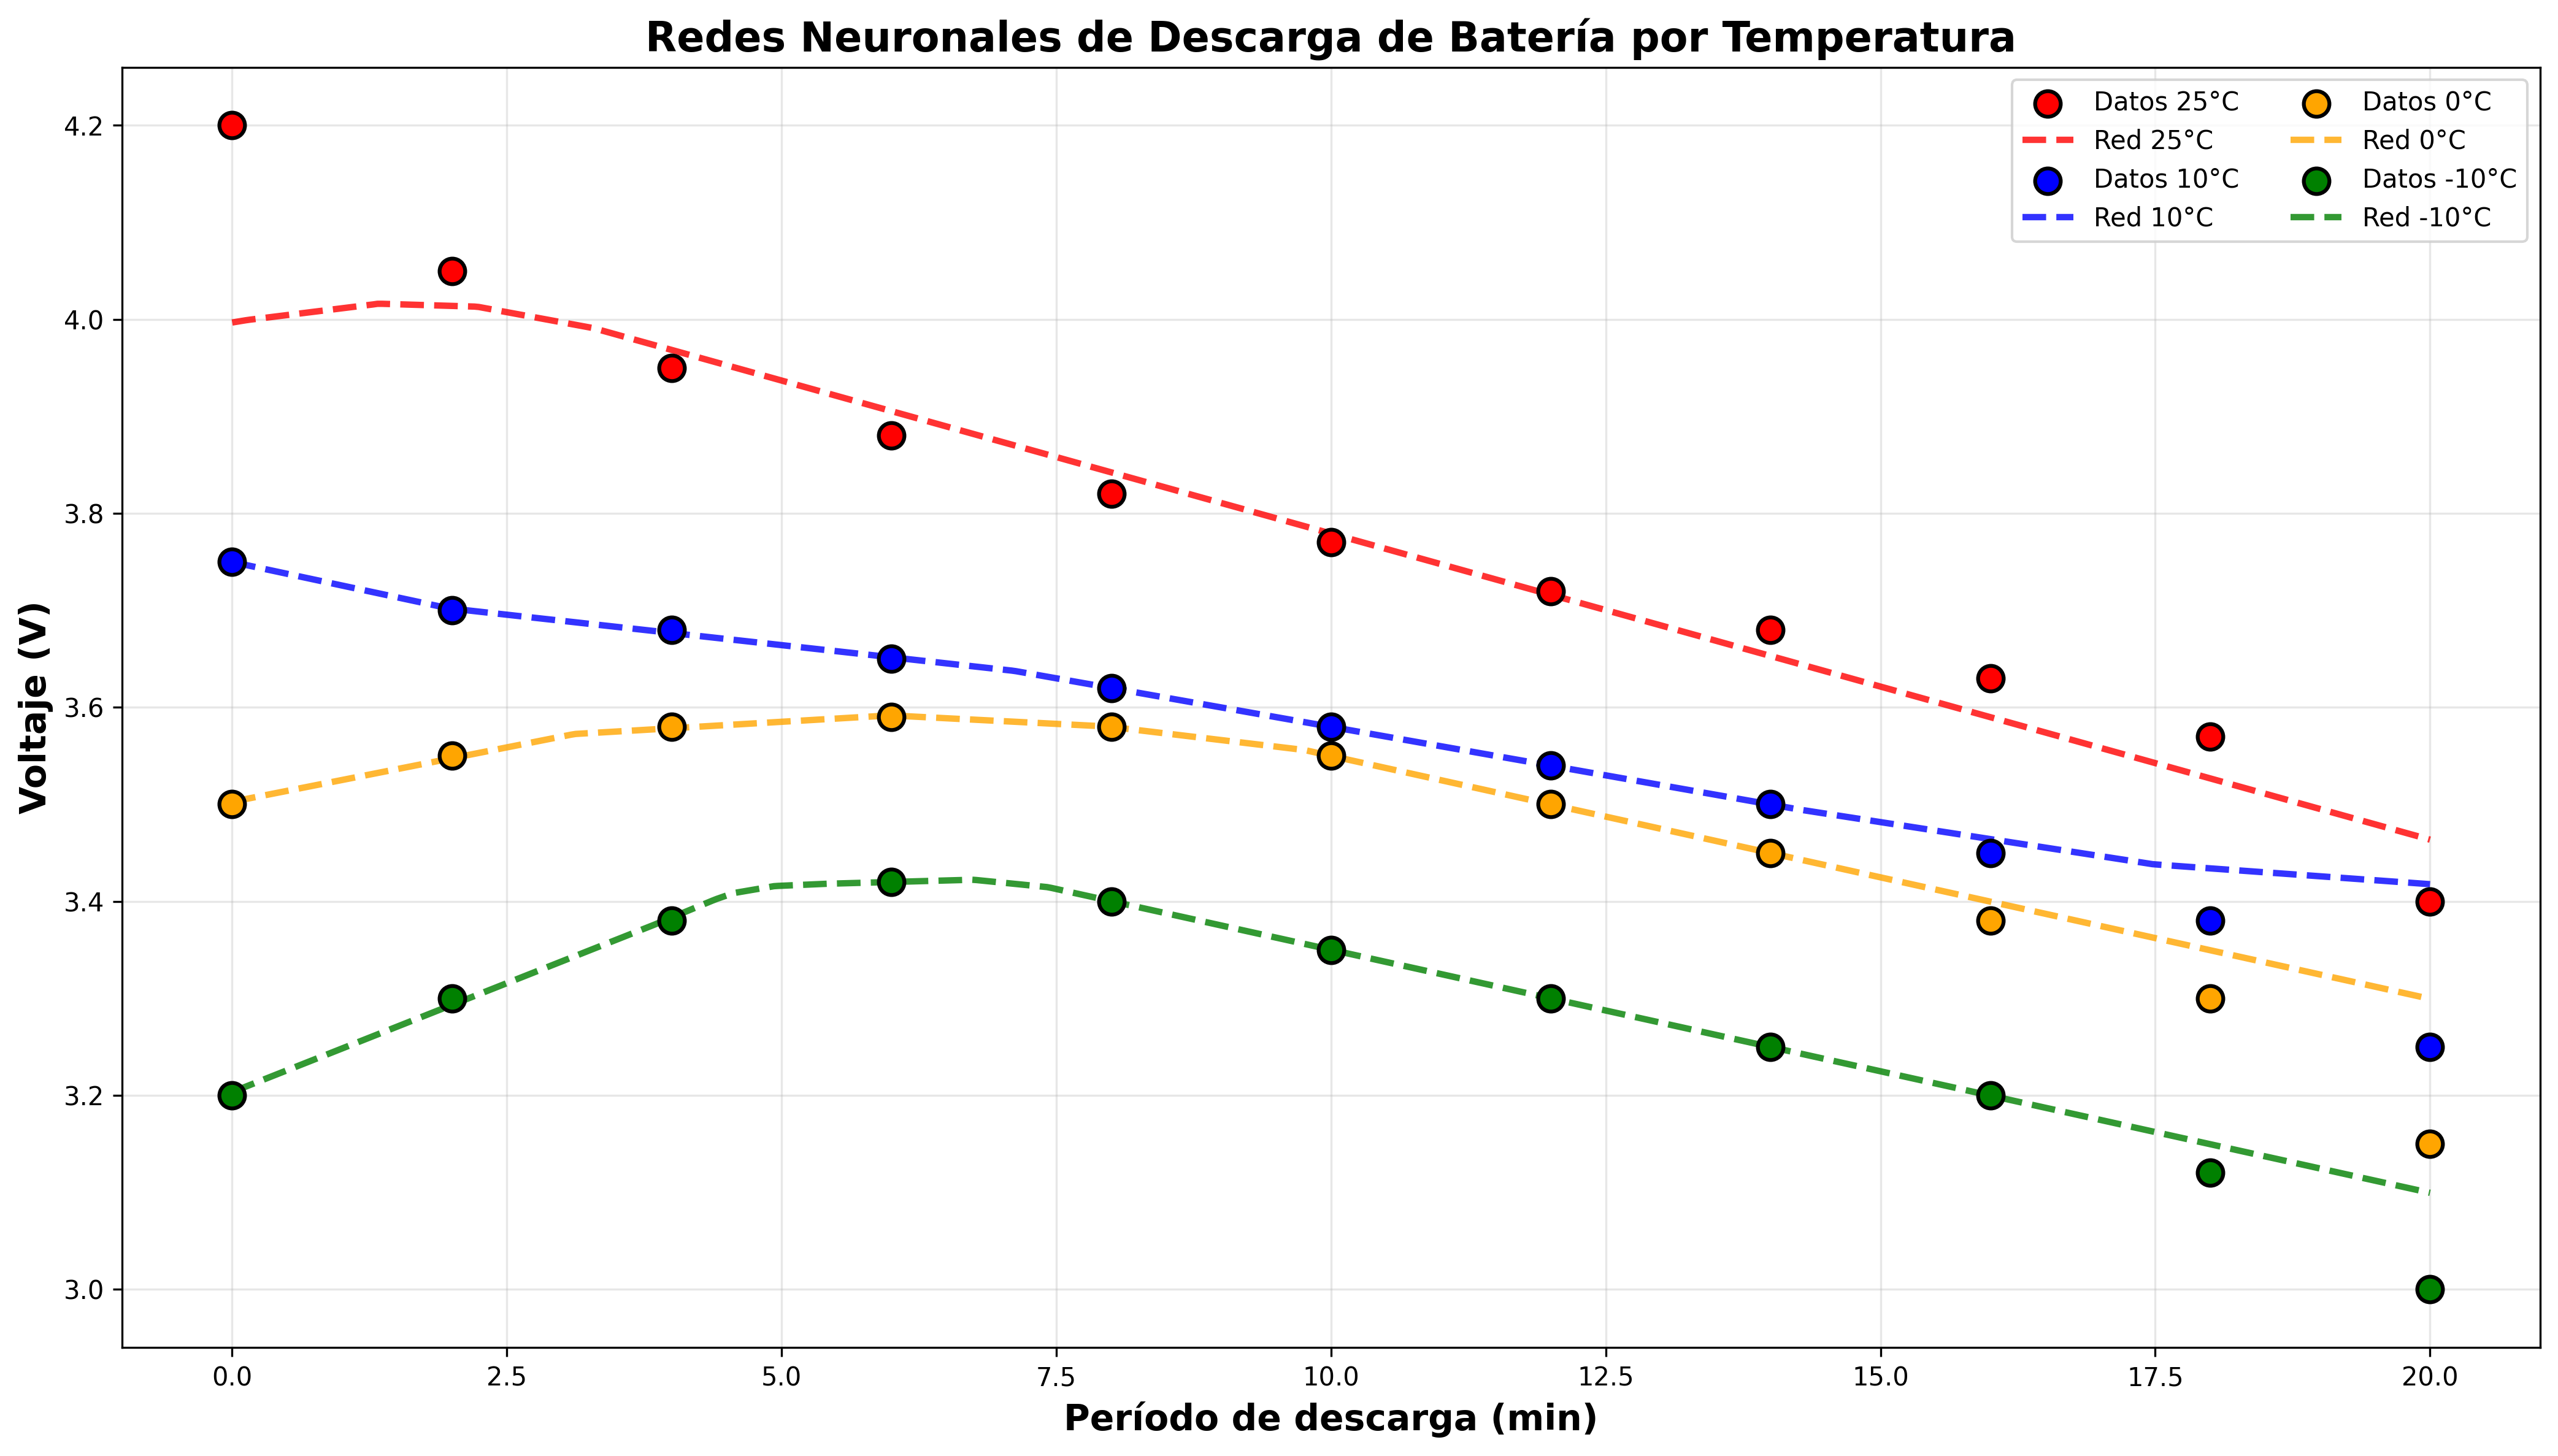
\includegraphics[width=\linewidth]{problema_1_todas_redes.png}
	\caption{Todas las redes neuronales de descarga de bater\'ia por temperatura. Los puntos representan los datos reales y las l\'ineas punteadas las predicciones de las redes neuronales.}
	\label{fig:p1_todas}
\end{figure*}

La Figura~\ref{fig:p1_todas} muestra las cuatro redes neuronales graficadas conjuntamente. Cada red captura correctamente la tendencia de descarga para su temperatura correspondiente.

\begin{figure}[H]\centering
	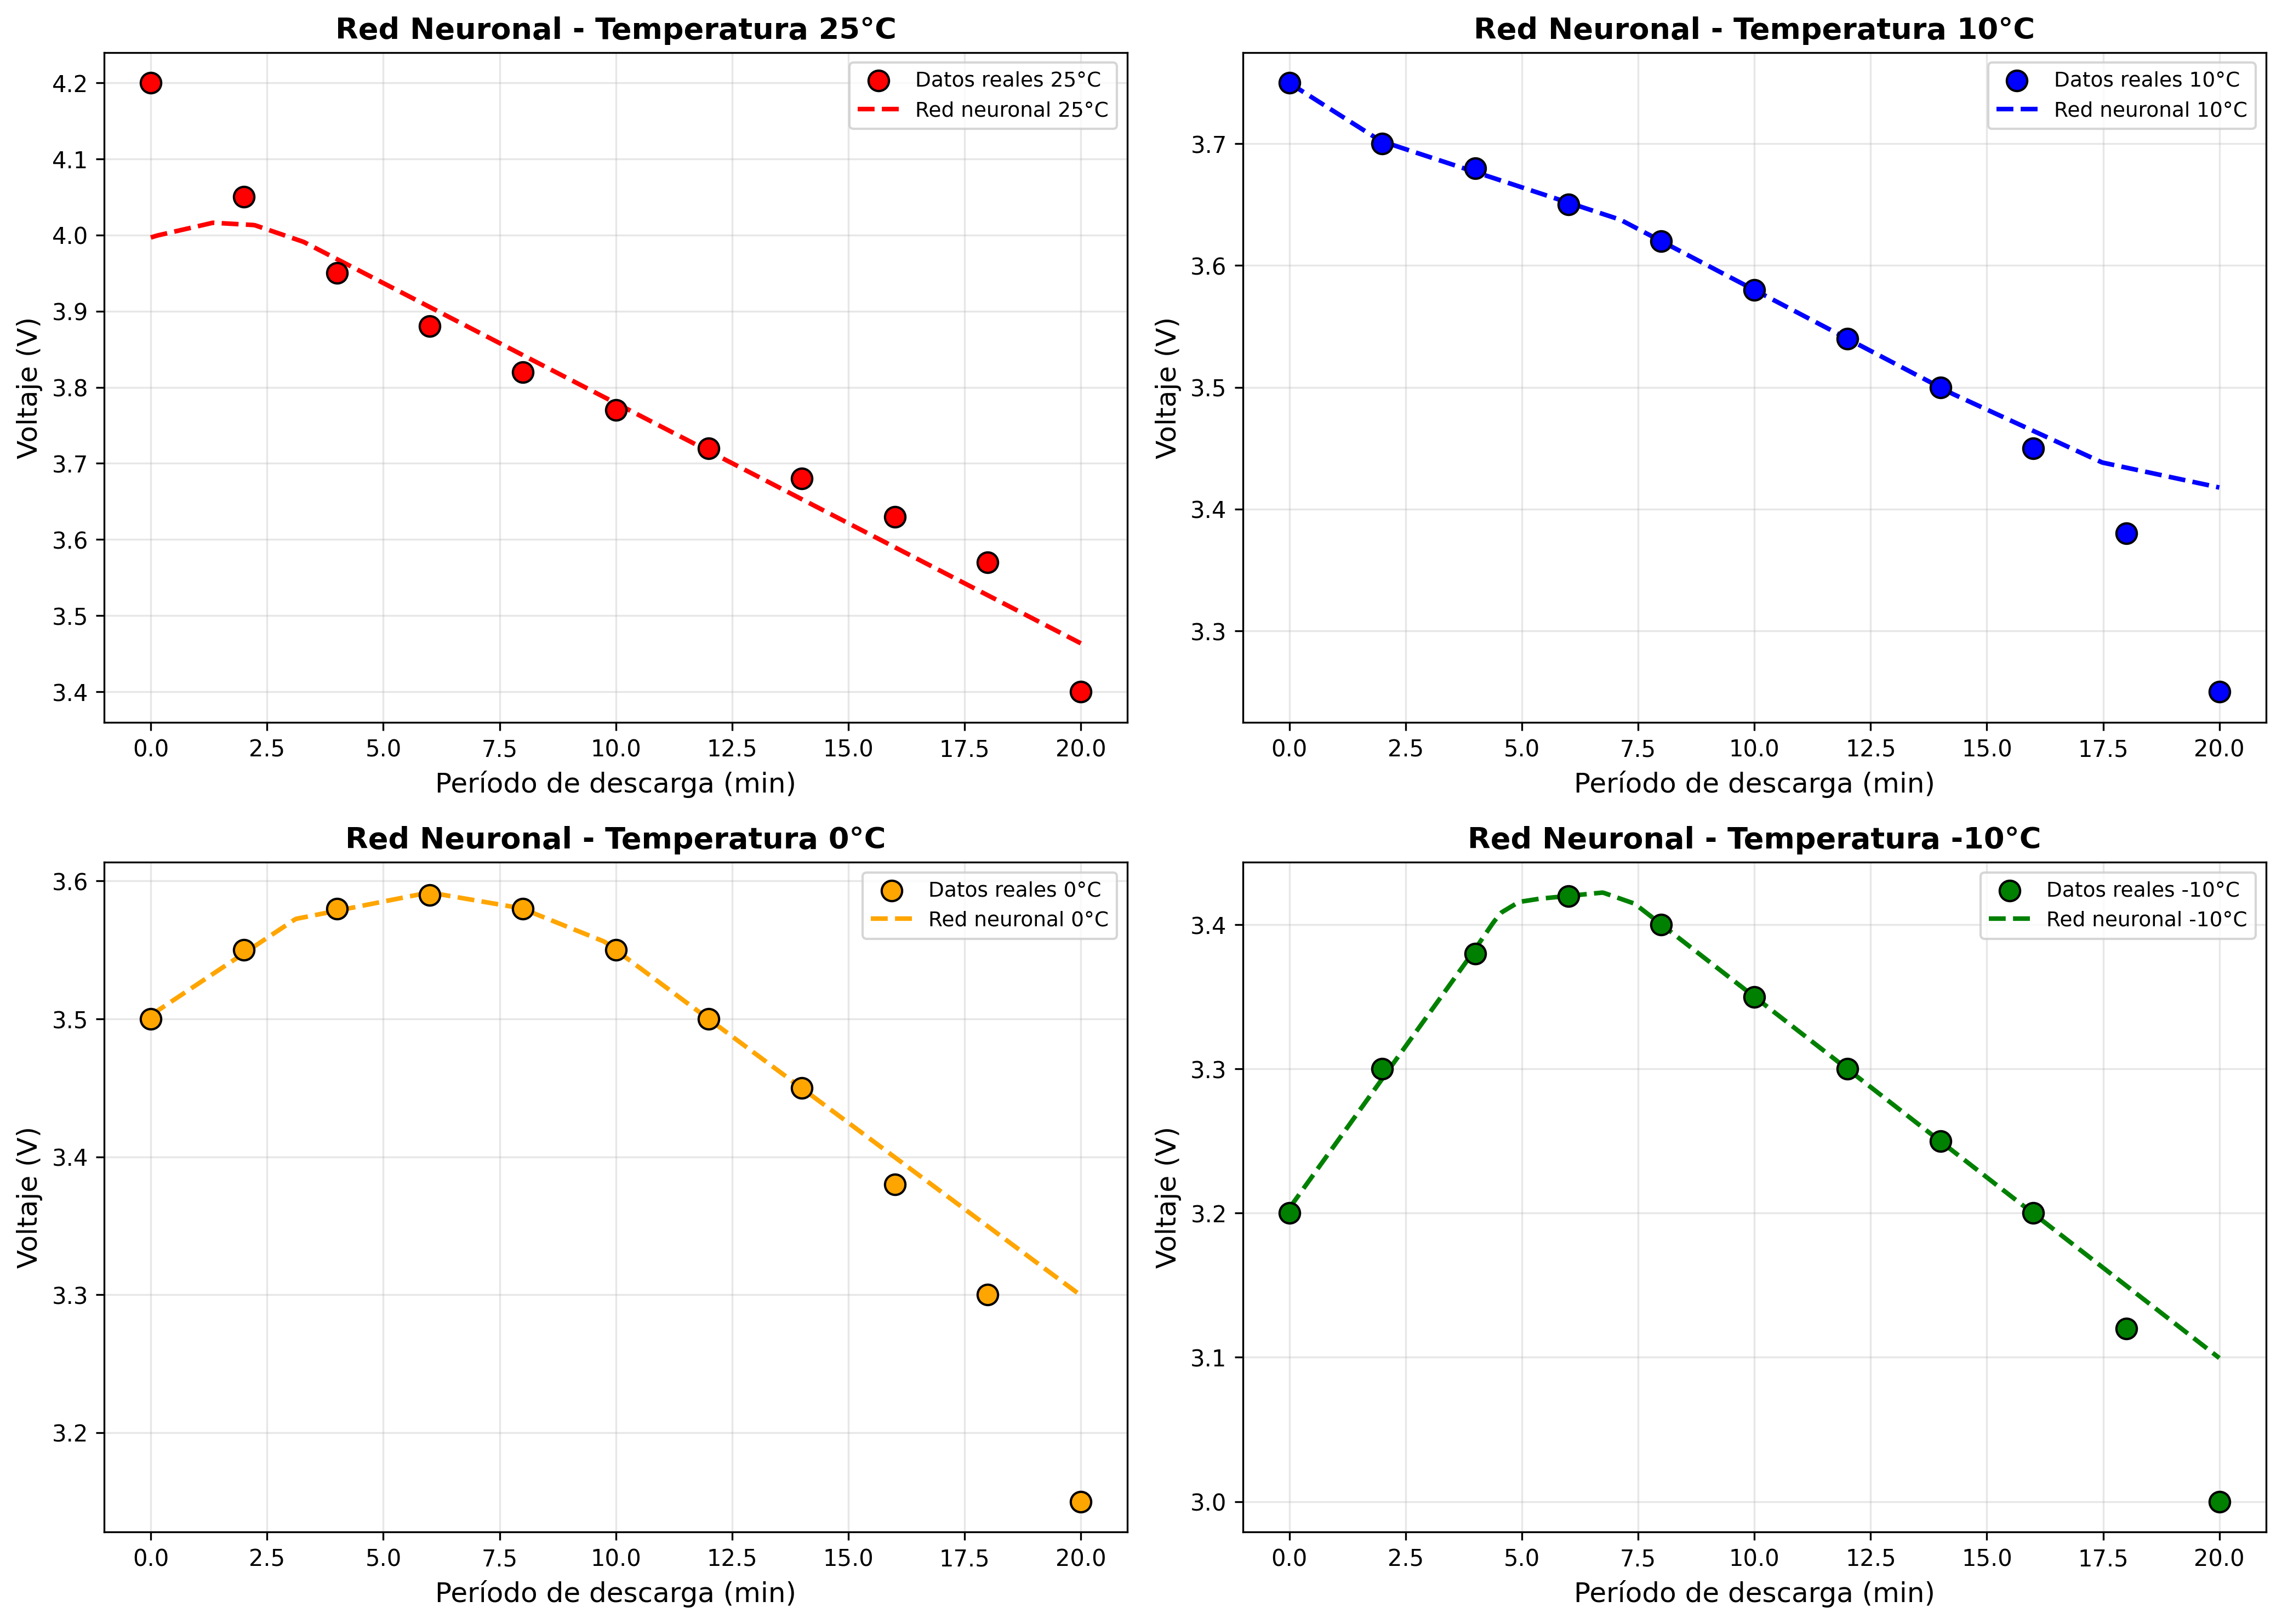
\includegraphics[width=\linewidth]{problema_1_individual.png}
	\caption{Ajuste individual de cada red neuronal por temperatura.}
	\label{fig:p1_individual}
\end{figure}

\begin{figure}[H]\centering
	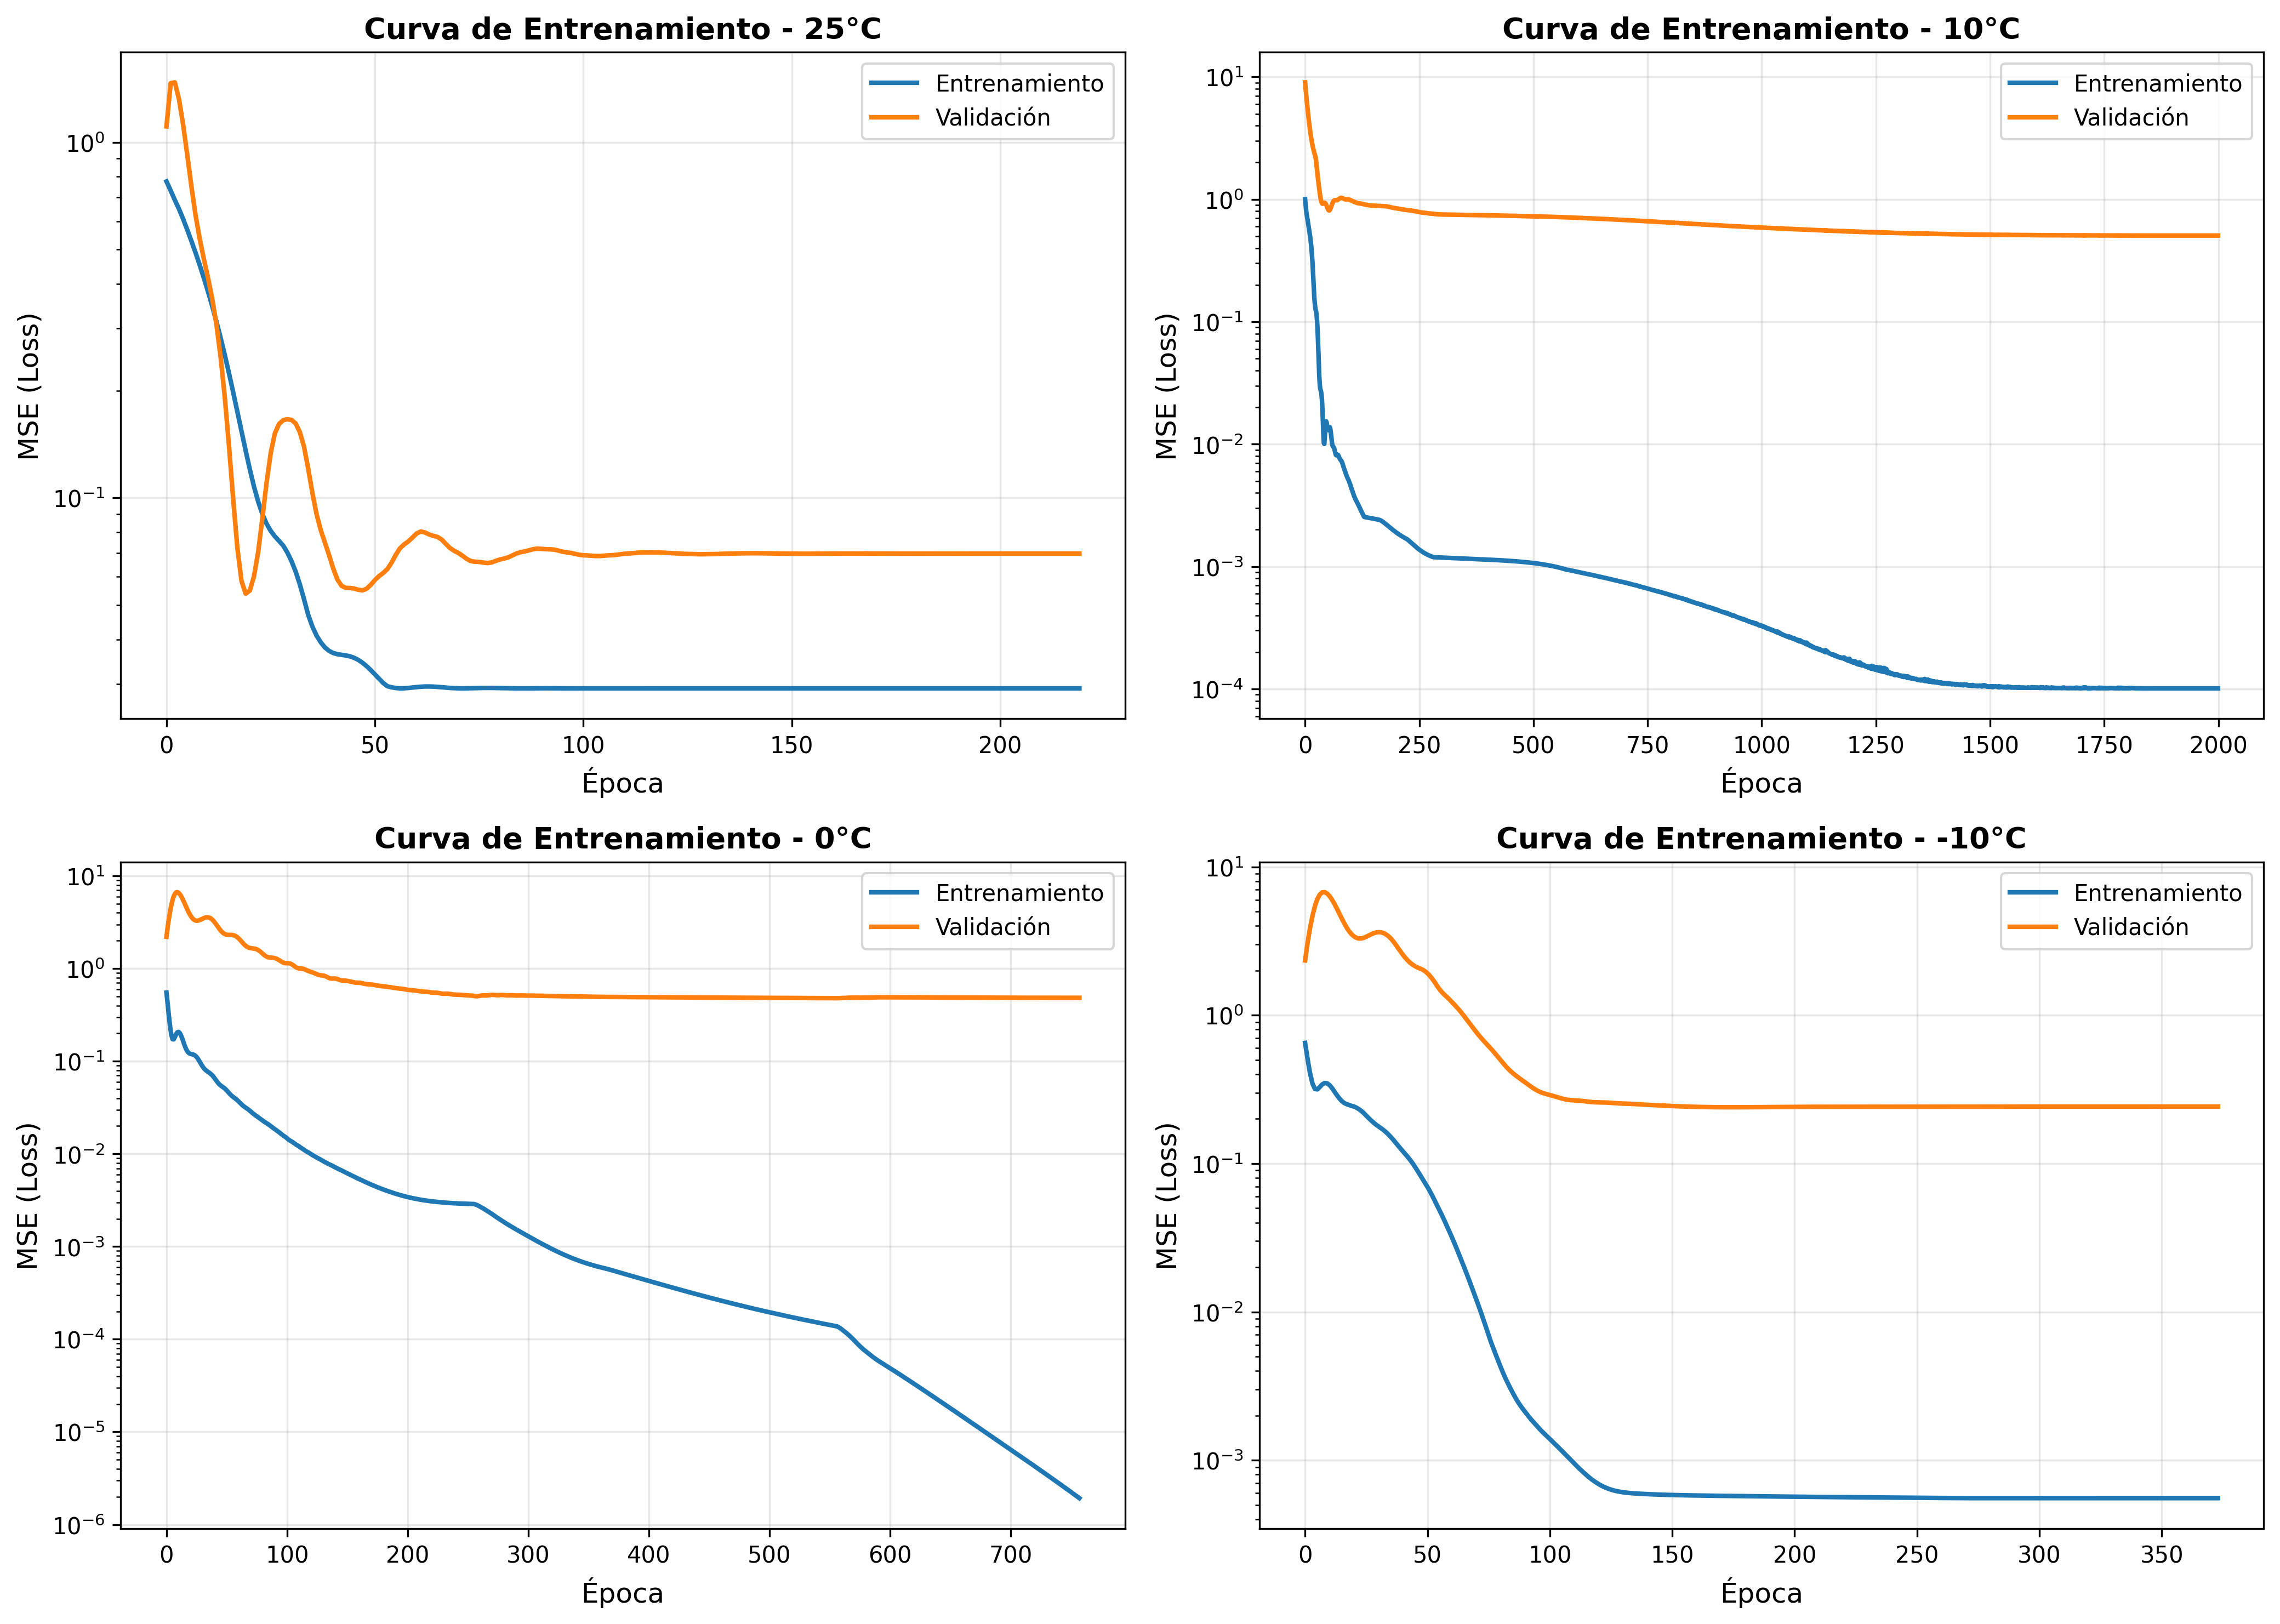
\includegraphics[width=\linewidth]{problema_1_loss.png}
	\caption{Curvas de entrenamiento (p\'erdida MSE) para cada temperatura.}
	\label{fig:p1_loss}
\end{figure}

\begin{figure}[H]\centering
	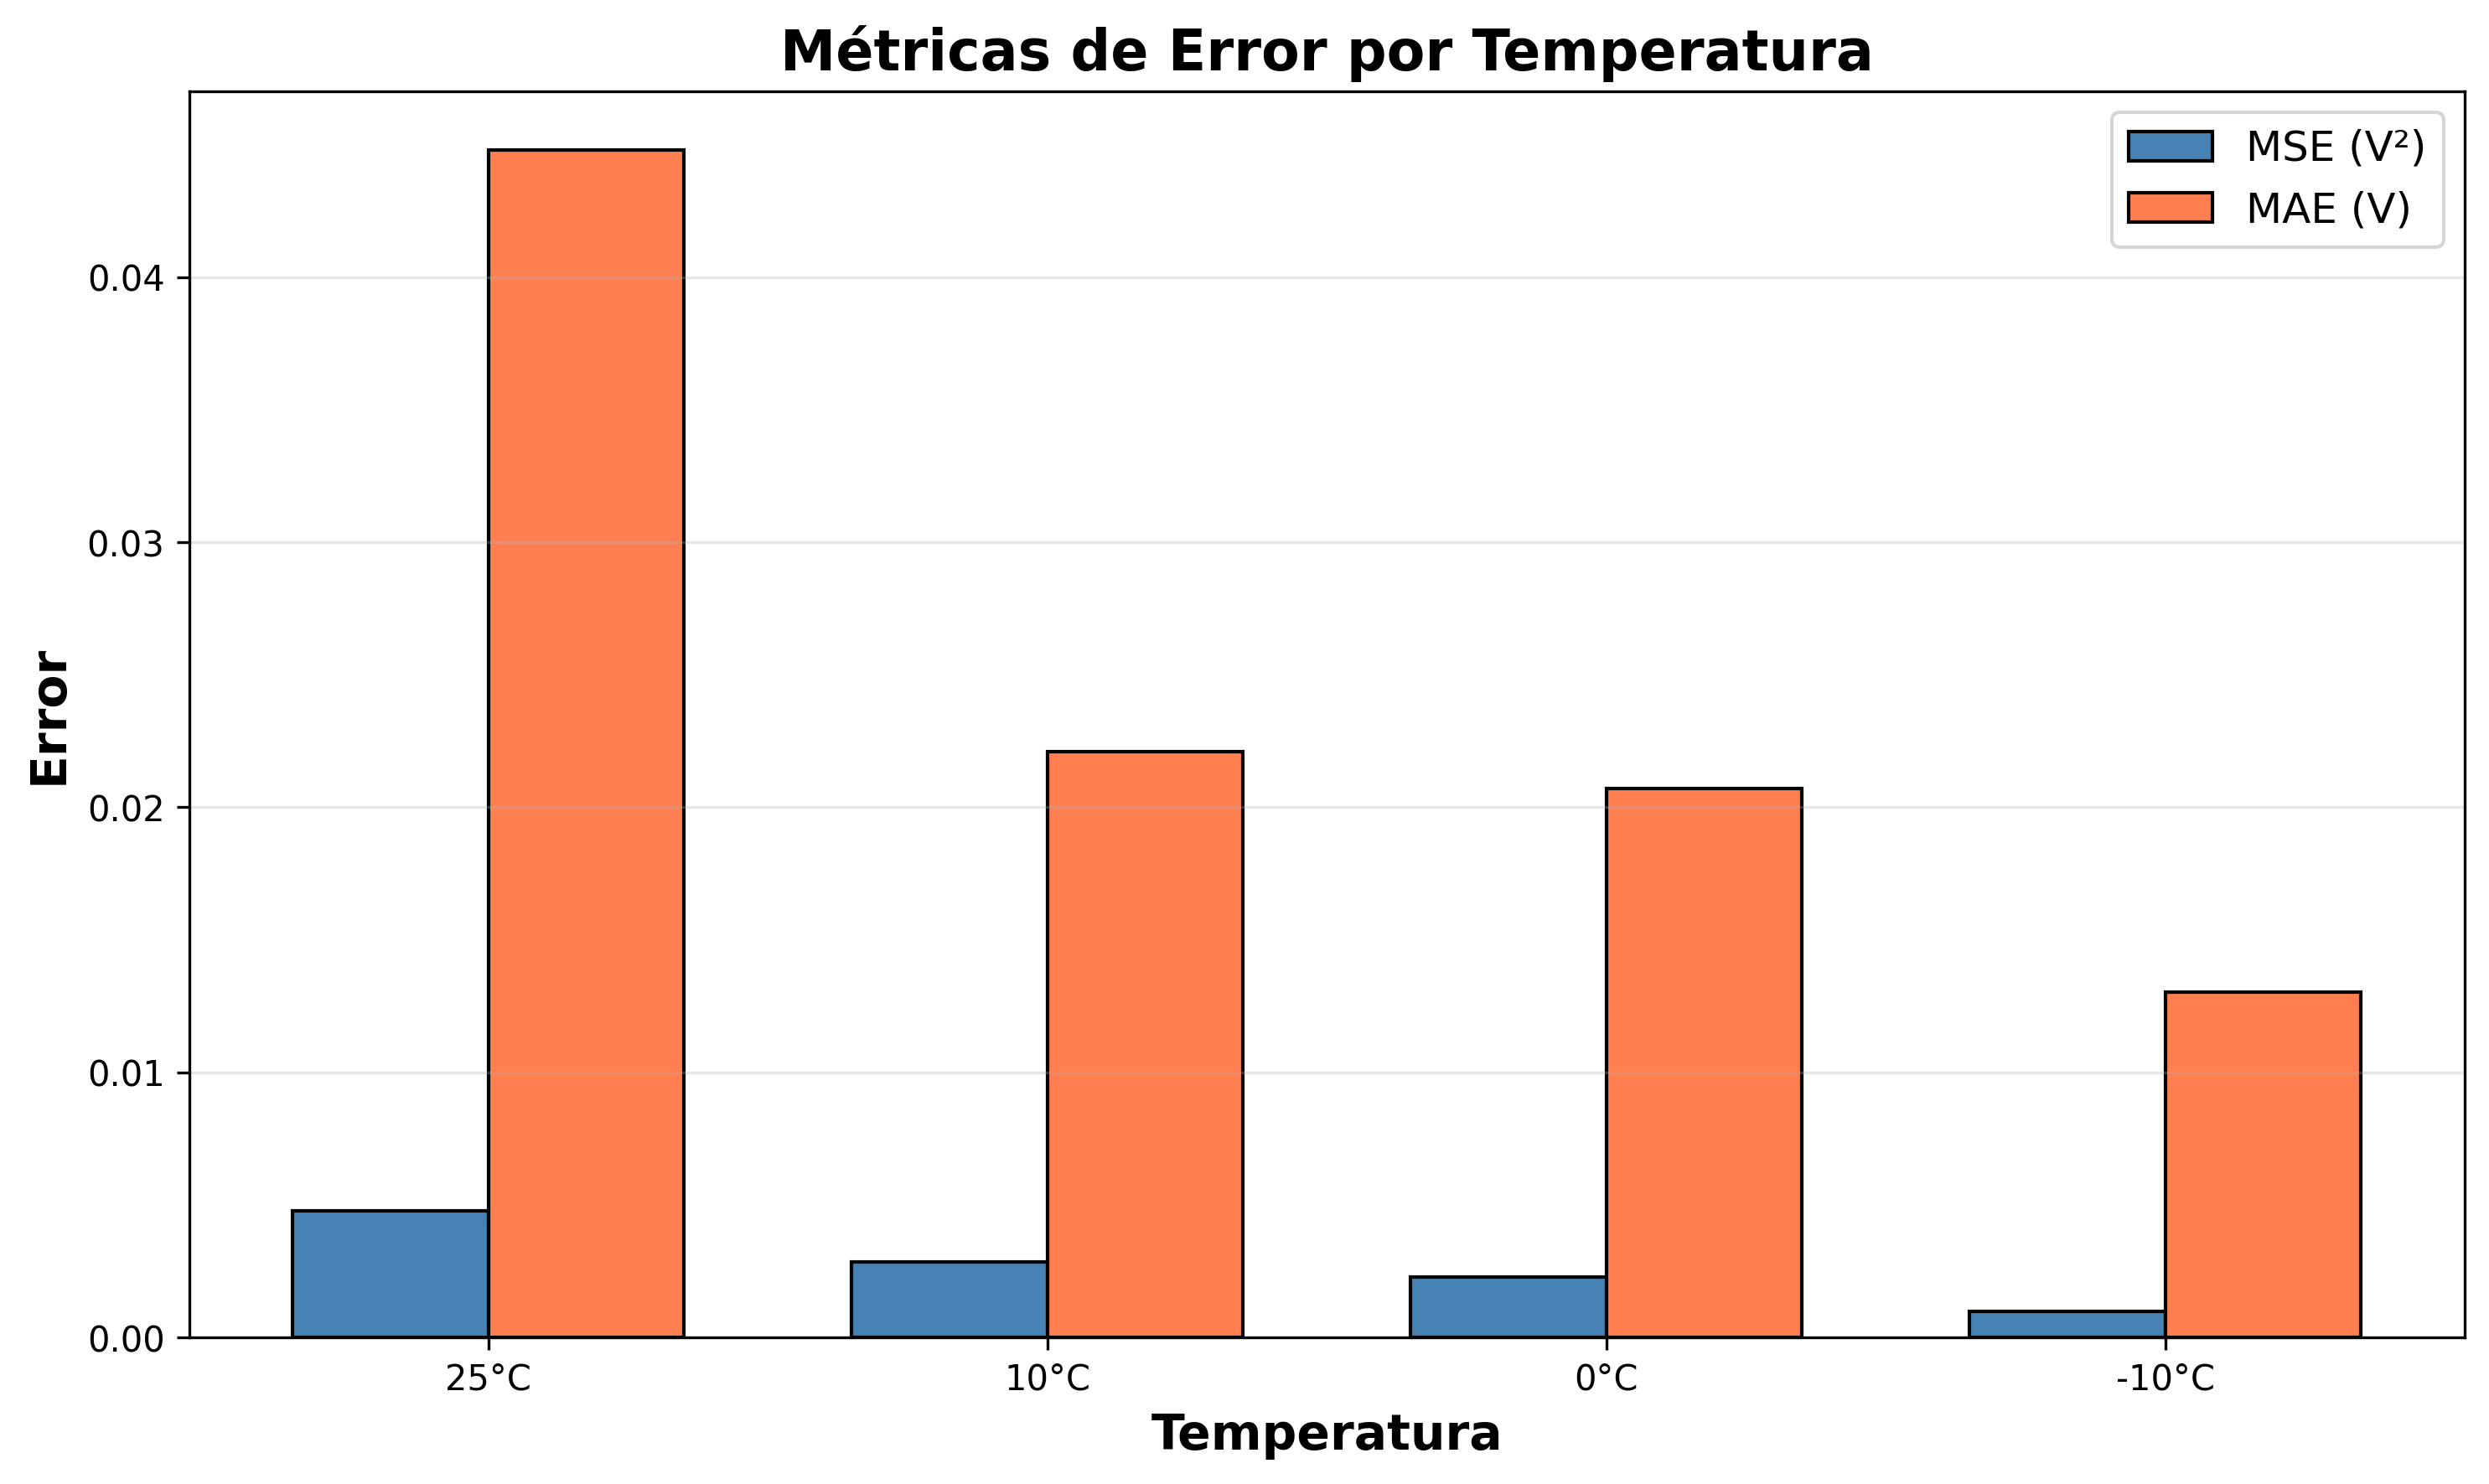
\includegraphics[width=\linewidth]{problema_1_errores.png}
	\caption{M\'etricas de error (MSE y MAE) por temperatura.}
	\label{fig:p1_errores}
\end{figure}

%----------------------------------------------------------------------------------------

\section{Problema 2: Intersecci\'on de Curvas (30 Puntos)}

Se desarrollaron redes neuronales para aproximar seis pares de curvas y determinar sus puntos de intersecci\'on.

\subsection{Pares de Curvas}

Los seis pares de funciones analizados son:

\begin{enumerate}[noitemsep]
	\item[a)] $y = x^2 - 2x + 1$ \quad y \quad $y = -x^2 + 5x - 2$
	\item[b)] $y = x^2 + 1$ \quad y \quad $y = x + 1$
	\item[c)] $y = x^2 - 3x + 1$ \quad y \quad $y = x + 1$
	\item[d)] $y = 2 - x^2$ \quad y \quad $y = x^2$
	\item[e)] $y = 2x - x^2$ \quad y \quad $y = x - 2$
	\item[f)] $y = x^2 - 4$ \quad y \quad $y = 3x - x^2 + 1$
\end{enumerate}

\subsection{Arquitectura de la Red}

Para cada funci\'on se entren\'o una red neuronal con:

\begin{itemize}[noitemsep]
	\item Capa de entrada: 1 neurona ($x$ normalizado)
	\item Capa oculta 1: 15 neuronas, activaci\'on ReLU
	\item Capa oculta 2: 15 neuronas, activaci\'on ReLU
	\item Capa de salida: 1 neurona, activaci\'on lineal
\end{itemize}

Se generaron 500 puntos sint\'eticos en el rango $[-5, 5]$, con Adam (lr=0.005), 1500 \'epocas y parada temprana. Los puntos de intersecci\'on se calcularon usando \texttt{scipy.optimize.fsolve}.

\subsection{Resultados}

\begin{figure*}[ht]\centering
	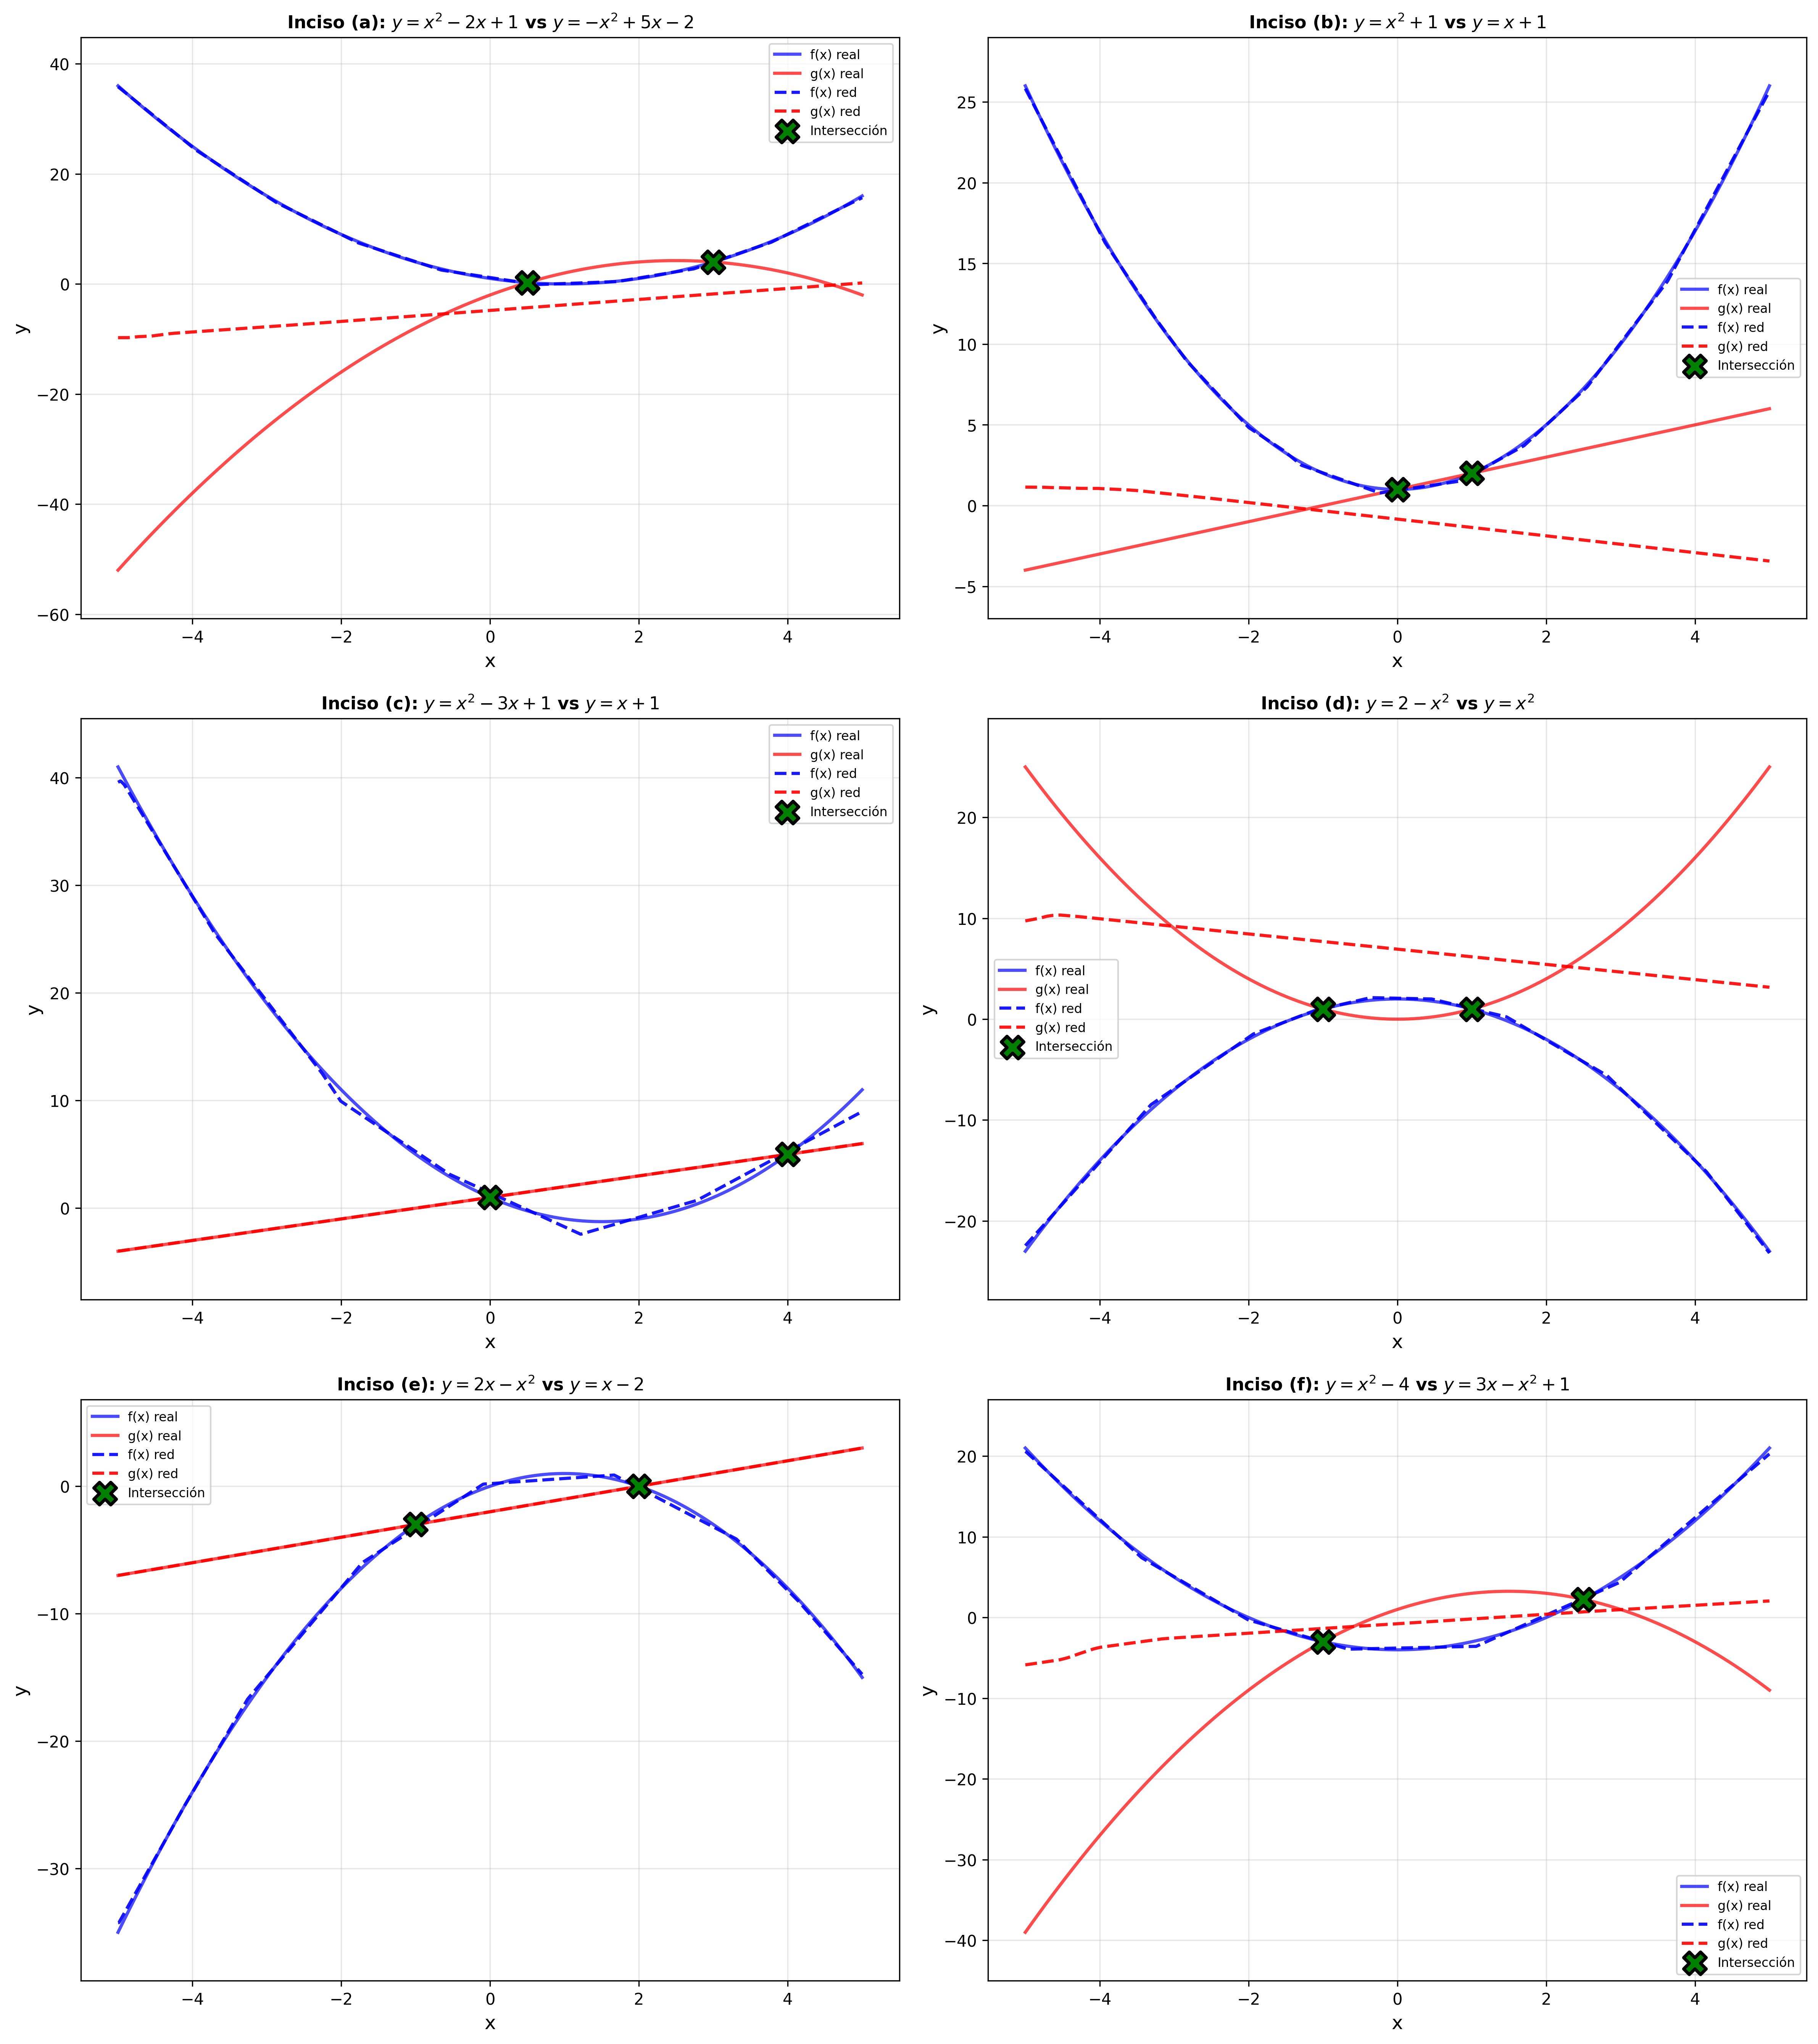
\includegraphics[width=\linewidth]{problema_2_incisos.png}
	\caption{Aproximaci\'on por redes neuronales de los seis pares de curvas. Las l\'ineas s\'olidas son las funciones reales, las punteadas las predicciones de la red. Los marcadores verdes indican los puntos de intersecci\'on.}
	\label{fig:p2_incisos}
\end{figure*}

\begin{figure*}[ht]\centering
	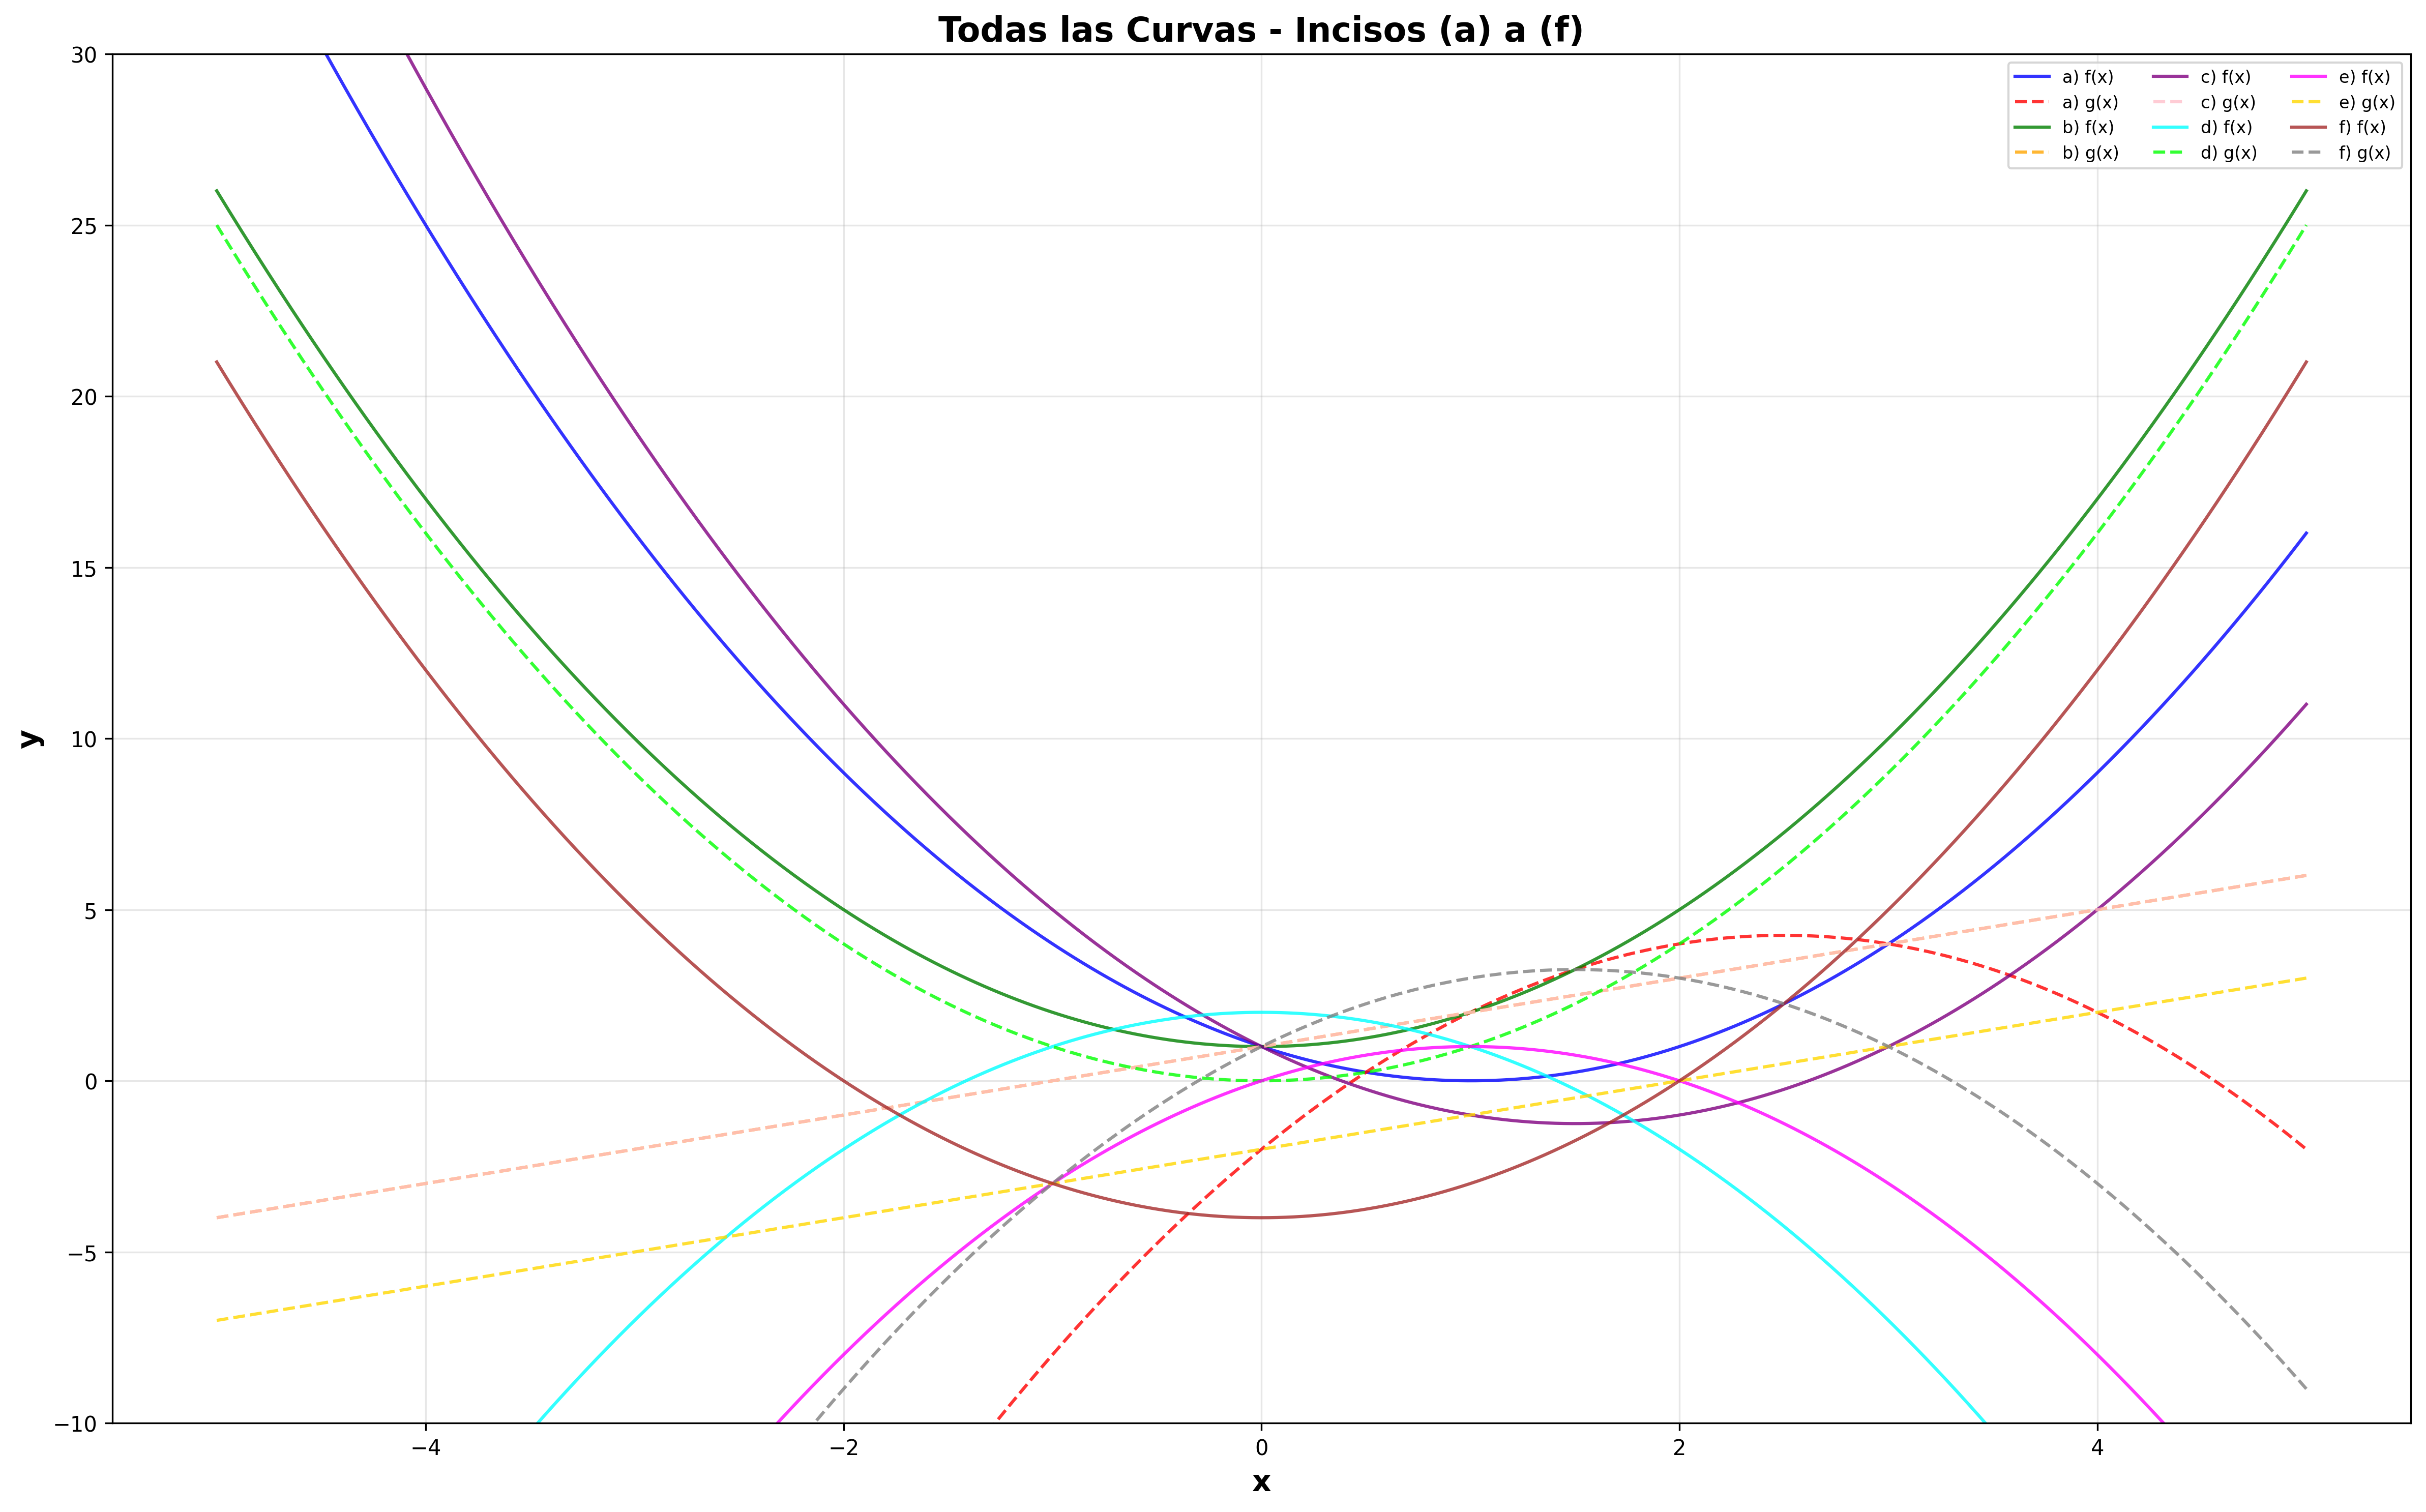
\includegraphics[width=\linewidth]{problema_2_todas_curvas.png}
	\caption{Todas las curvas de los seis incisos graficadas en una sola imagen.}
	\label{fig:p2_todas}
\end{figure*}

\begin{figure}[H]\centering
	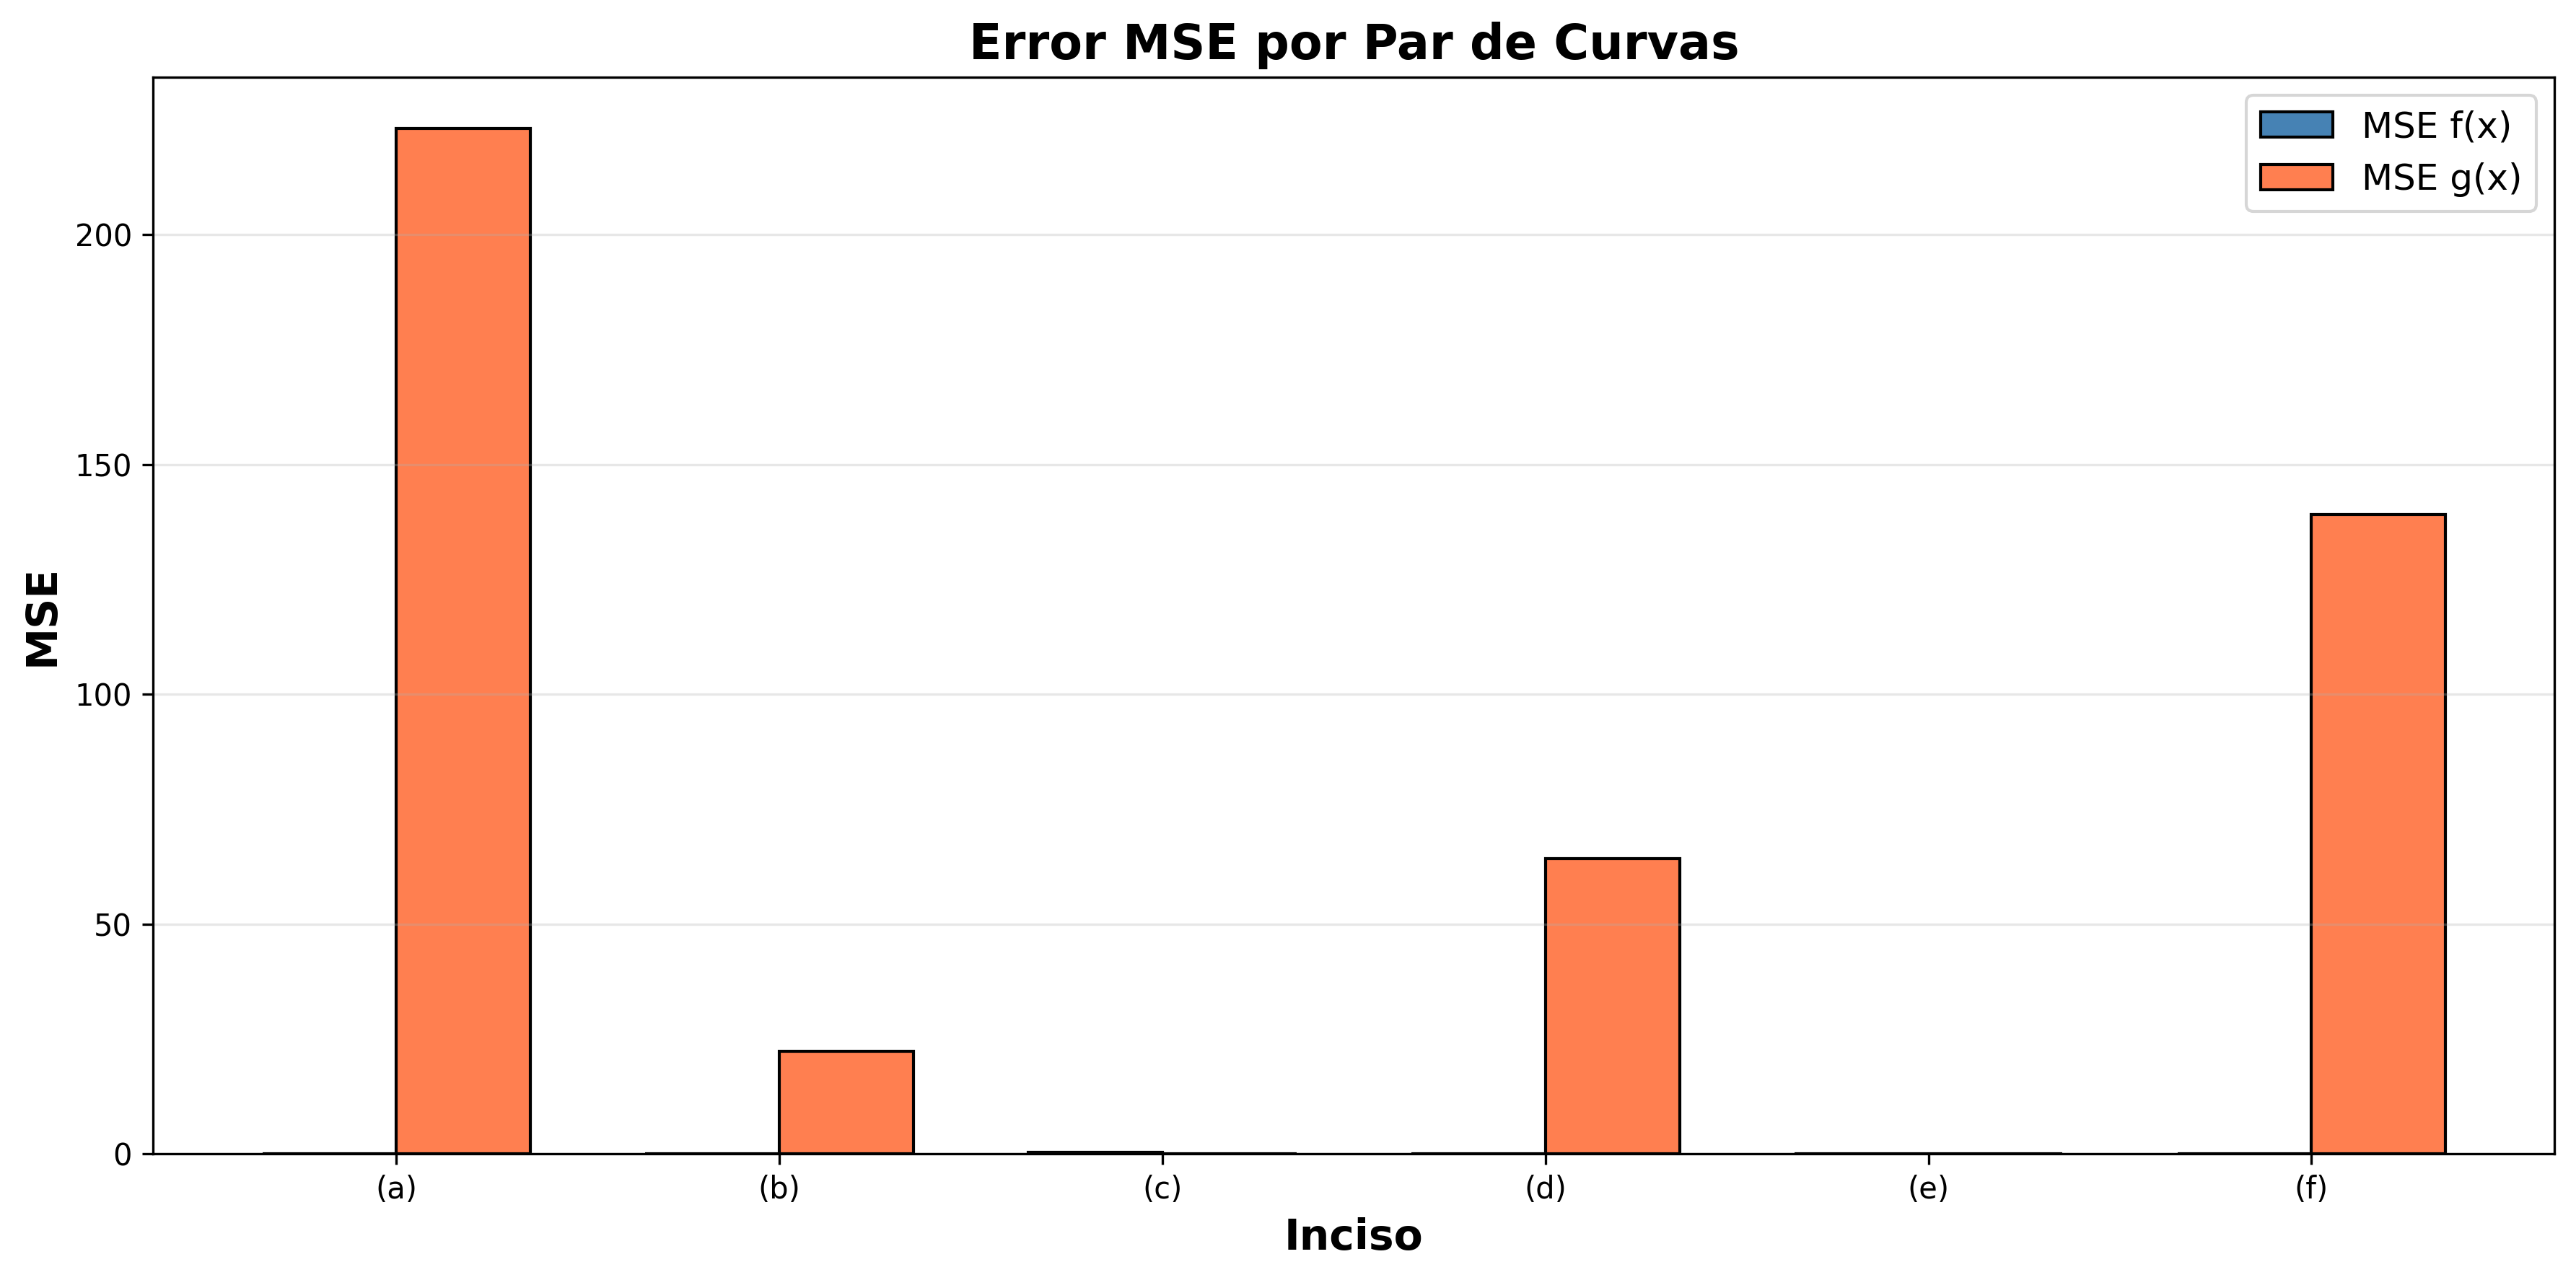
\includegraphics[width=\linewidth]{problema_2_errores.png}
	\caption{Error MSE por par de curvas para $f(x)$ y $g(x)$.}
	\label{fig:p2_errores}
\end{figure}

%----------------------------------------------------------------------------------------

\section{Problema 3: Choque de Proyectiles (30 Puntos)}

Se analiza la colisi\'on de dos proyectiles lanzados desde posiciones opuestas, determinando el tiempo y posici\'on de impacto tanto anal\'iticamente como mediante redes neuronales.

\subsection{Condiciones Iniciales}

\begin{itemize}[noitemsep]
	\item \textbf{Proyectil A}: $v_0 = 50$ m/s, $\theta = 30°$, $h_0 = 10$ m, $x_0 = 0$ m
	\item \textbf{Proyectil B}: $v_0 = 30\sqrt{2}$ m/s, $\theta = 45°$, $h_0 = 0$ m, $x_0 = 150$ m (disparado hacia A)
\end{itemize}

Las ecuaciones de movimiento para cada proyectil son:

\begin{equation}
	x_A(t) = v_{0A}\cos\theta_A \cdot t, \quad y_A(t) = h_{0A} + v_{0A}\sin\theta_A \cdot t - \frac{1}{2}gt^2
\end{equation}

\begin{equation}
	x_B(t) = x_{0B} - v_{0B}\cos\theta_B \cdot t, \quad y_B(t) = v_{0B}\sin\theta_B \cdot t - \frac{1}{2}gt^2
\end{equation}

El tiempo de impacto se obtiene resolviendo $x_A(t) = x_B(t)$ mediante \texttt{fsolve}, verificando que $y_A(t) = y_B(t)$ en dicho instante.

\subsection{Red Neuronal de Trayectoria}

Se entrenaron dos redes neuronales (una por proyectil) con arquitectura:

\begin{itemize}[noitemsep]
	\item Capa de entrada: 1 neurona (tiempo normalizado)
	\item Capa oculta 1: 20 neuronas, activaci\'on ReLU
	\item Capa oculta 2: 20 neuronas, activaci\'on ReLU
	\item Capa de salida: 2 neuronas ($x$, $y$), activaci\'on lineal
\end{itemize}

\subsection{Resultados}

\begin{figure*}[ht]\centering
	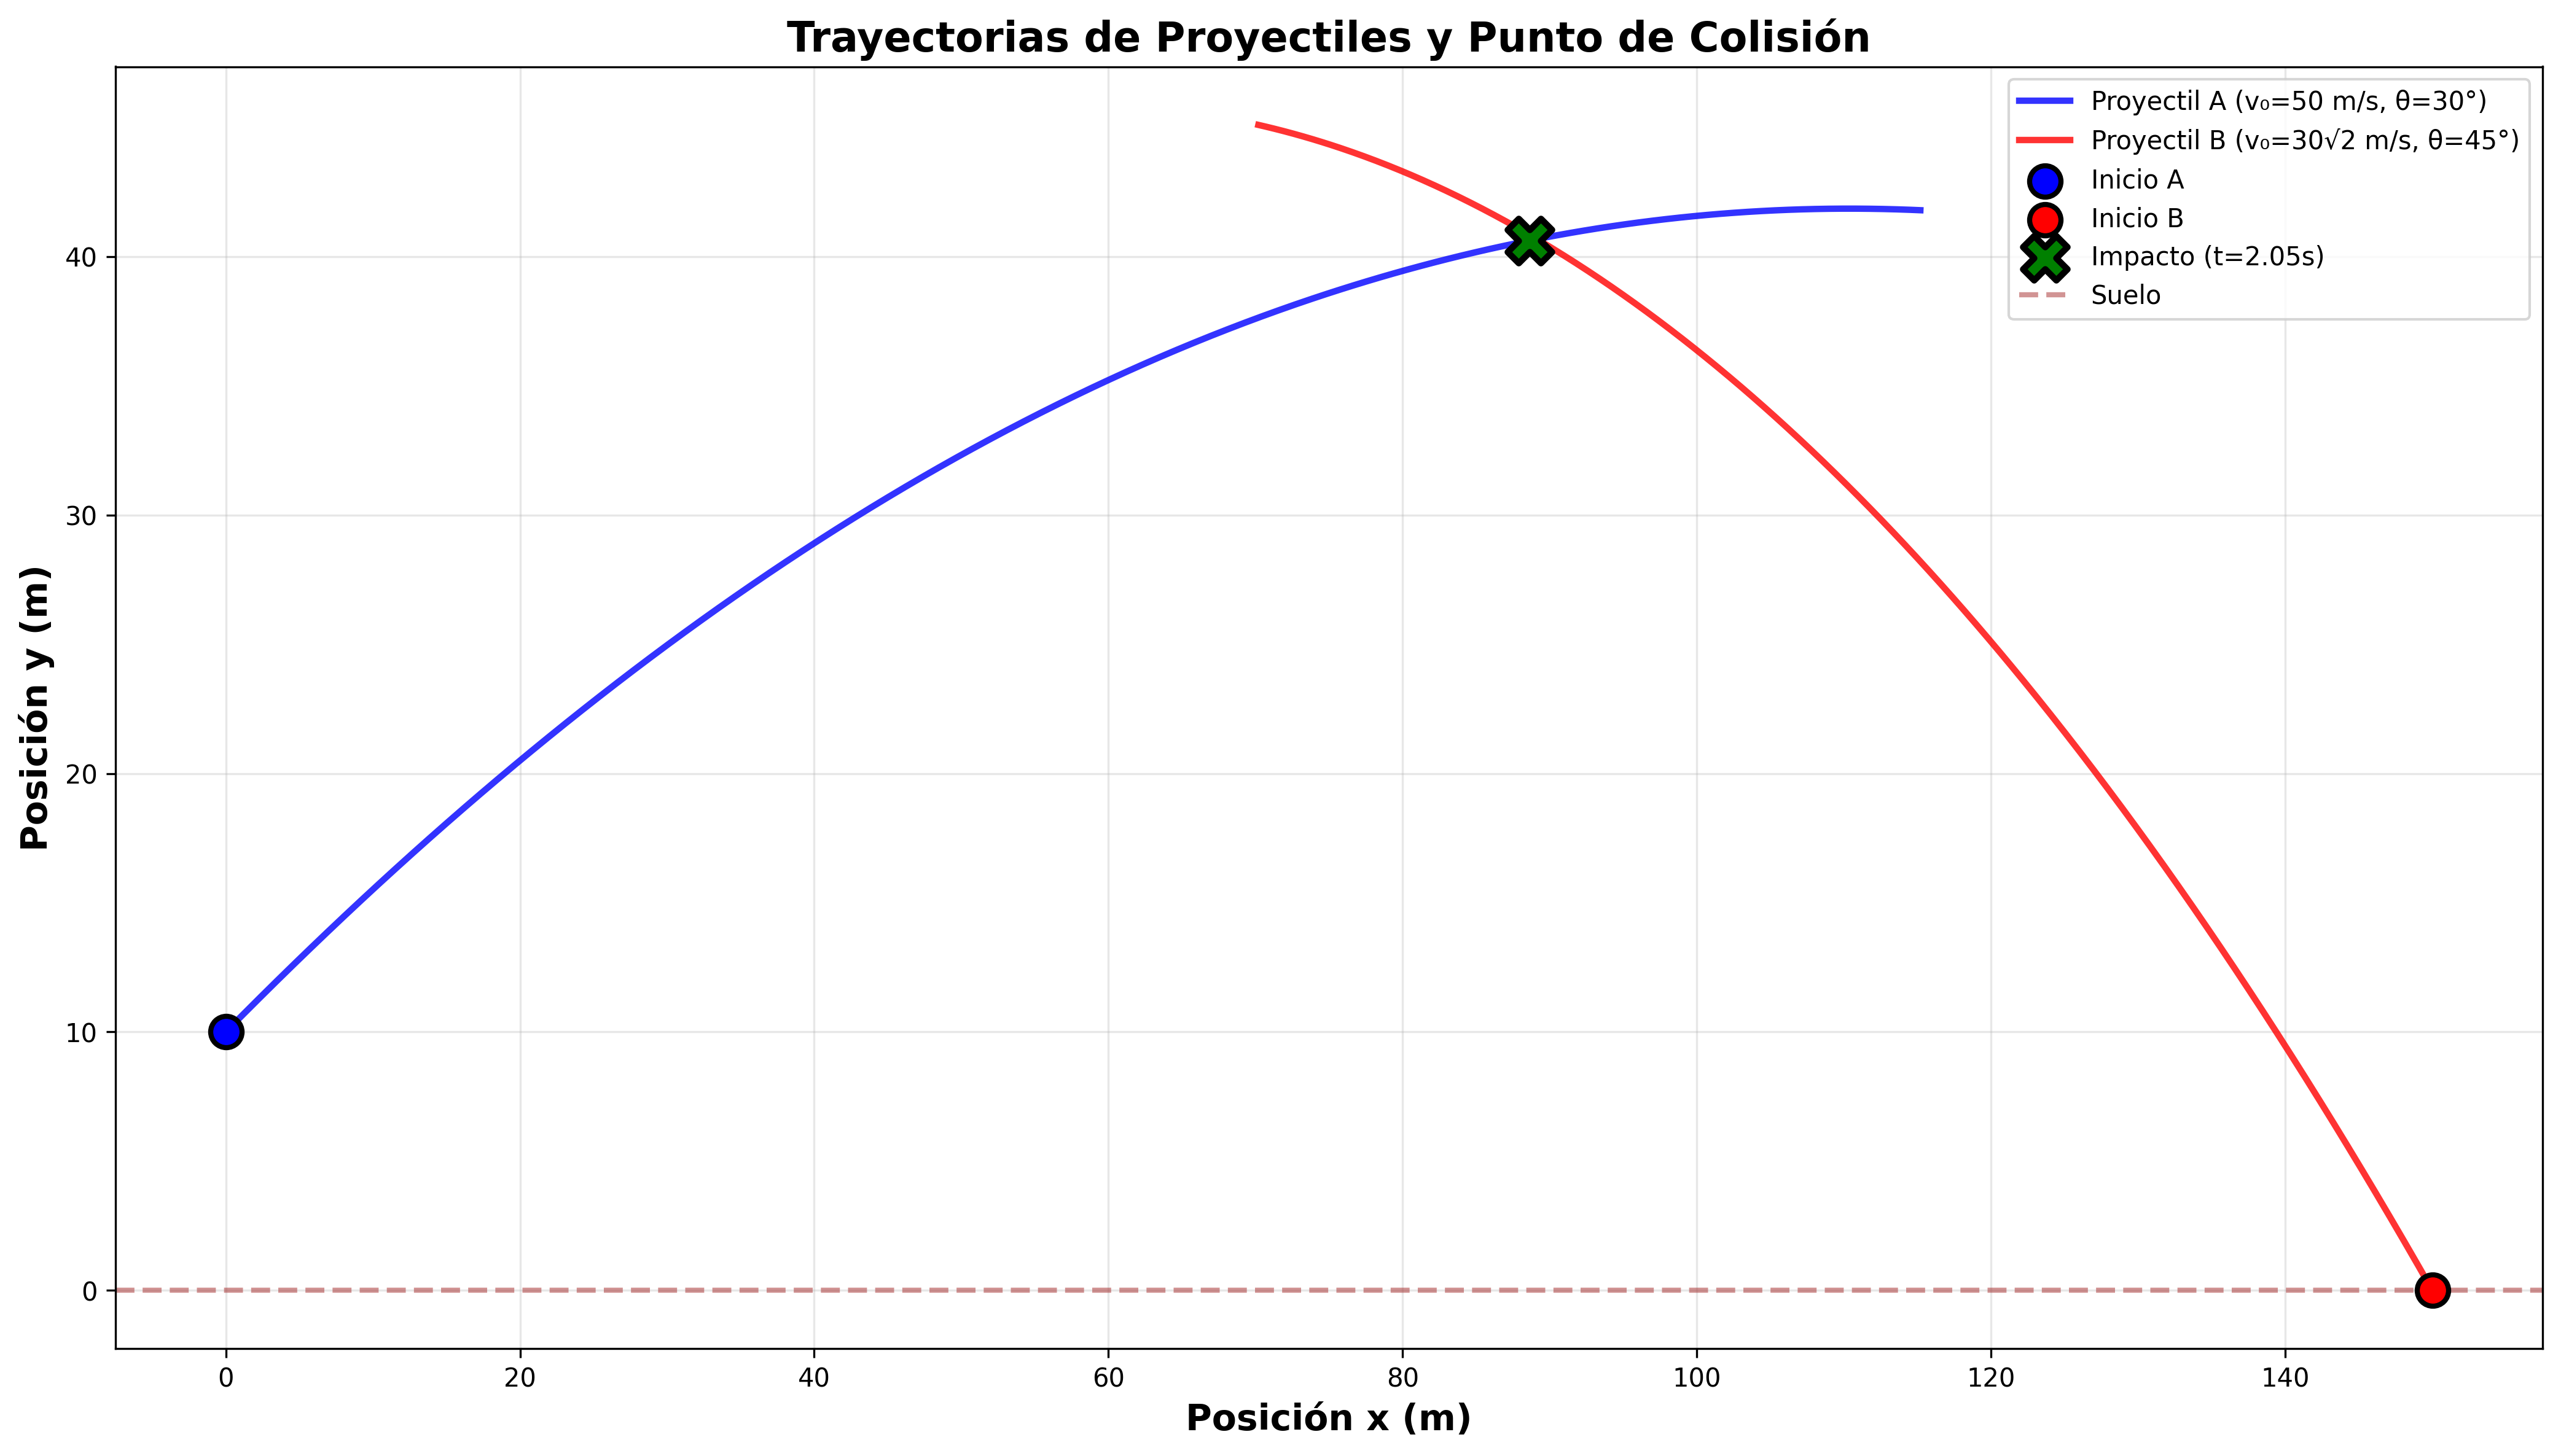
\includegraphics[width=\linewidth]{problema_3_trayectorias.png}
	\caption{Trayectorias de ambos proyectiles con el punto de colisi\'on marcado en verde.}
	\label{fig:p3_tray}
\end{figure*}

\begin{figure*}[ht]\centering
	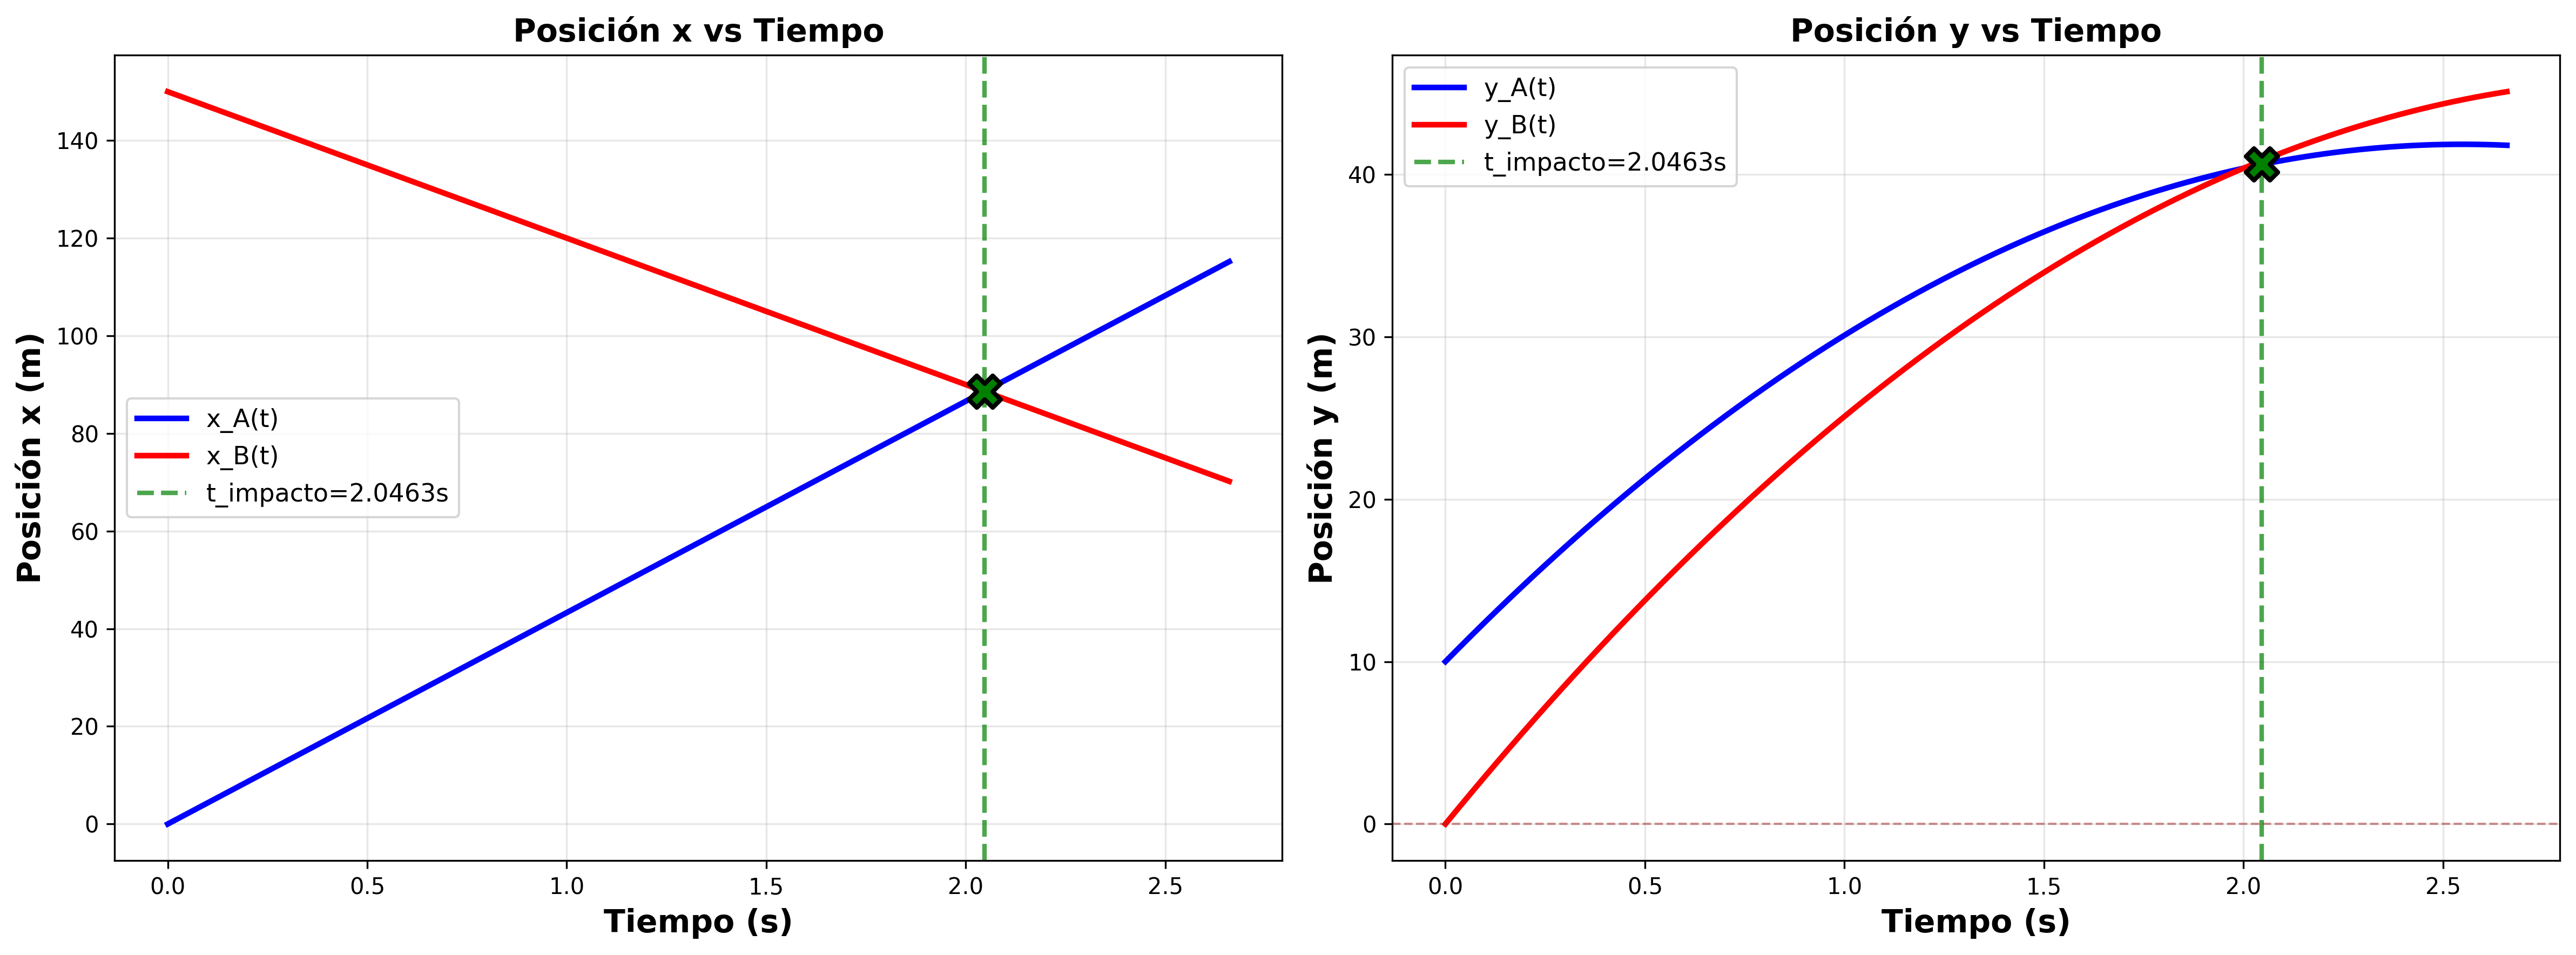
\includegraphics[width=\linewidth]{problema_3_posiciones_tiempo.png}
	\caption{Posiciones $x(t)$ e $y(t)$ de ambos proyectiles. La l\'inea vertical verde indica el tiempo de impacto.}
	\label{fig:p3_pos}
\end{figure*}

\begin{figure}[H]\centering
	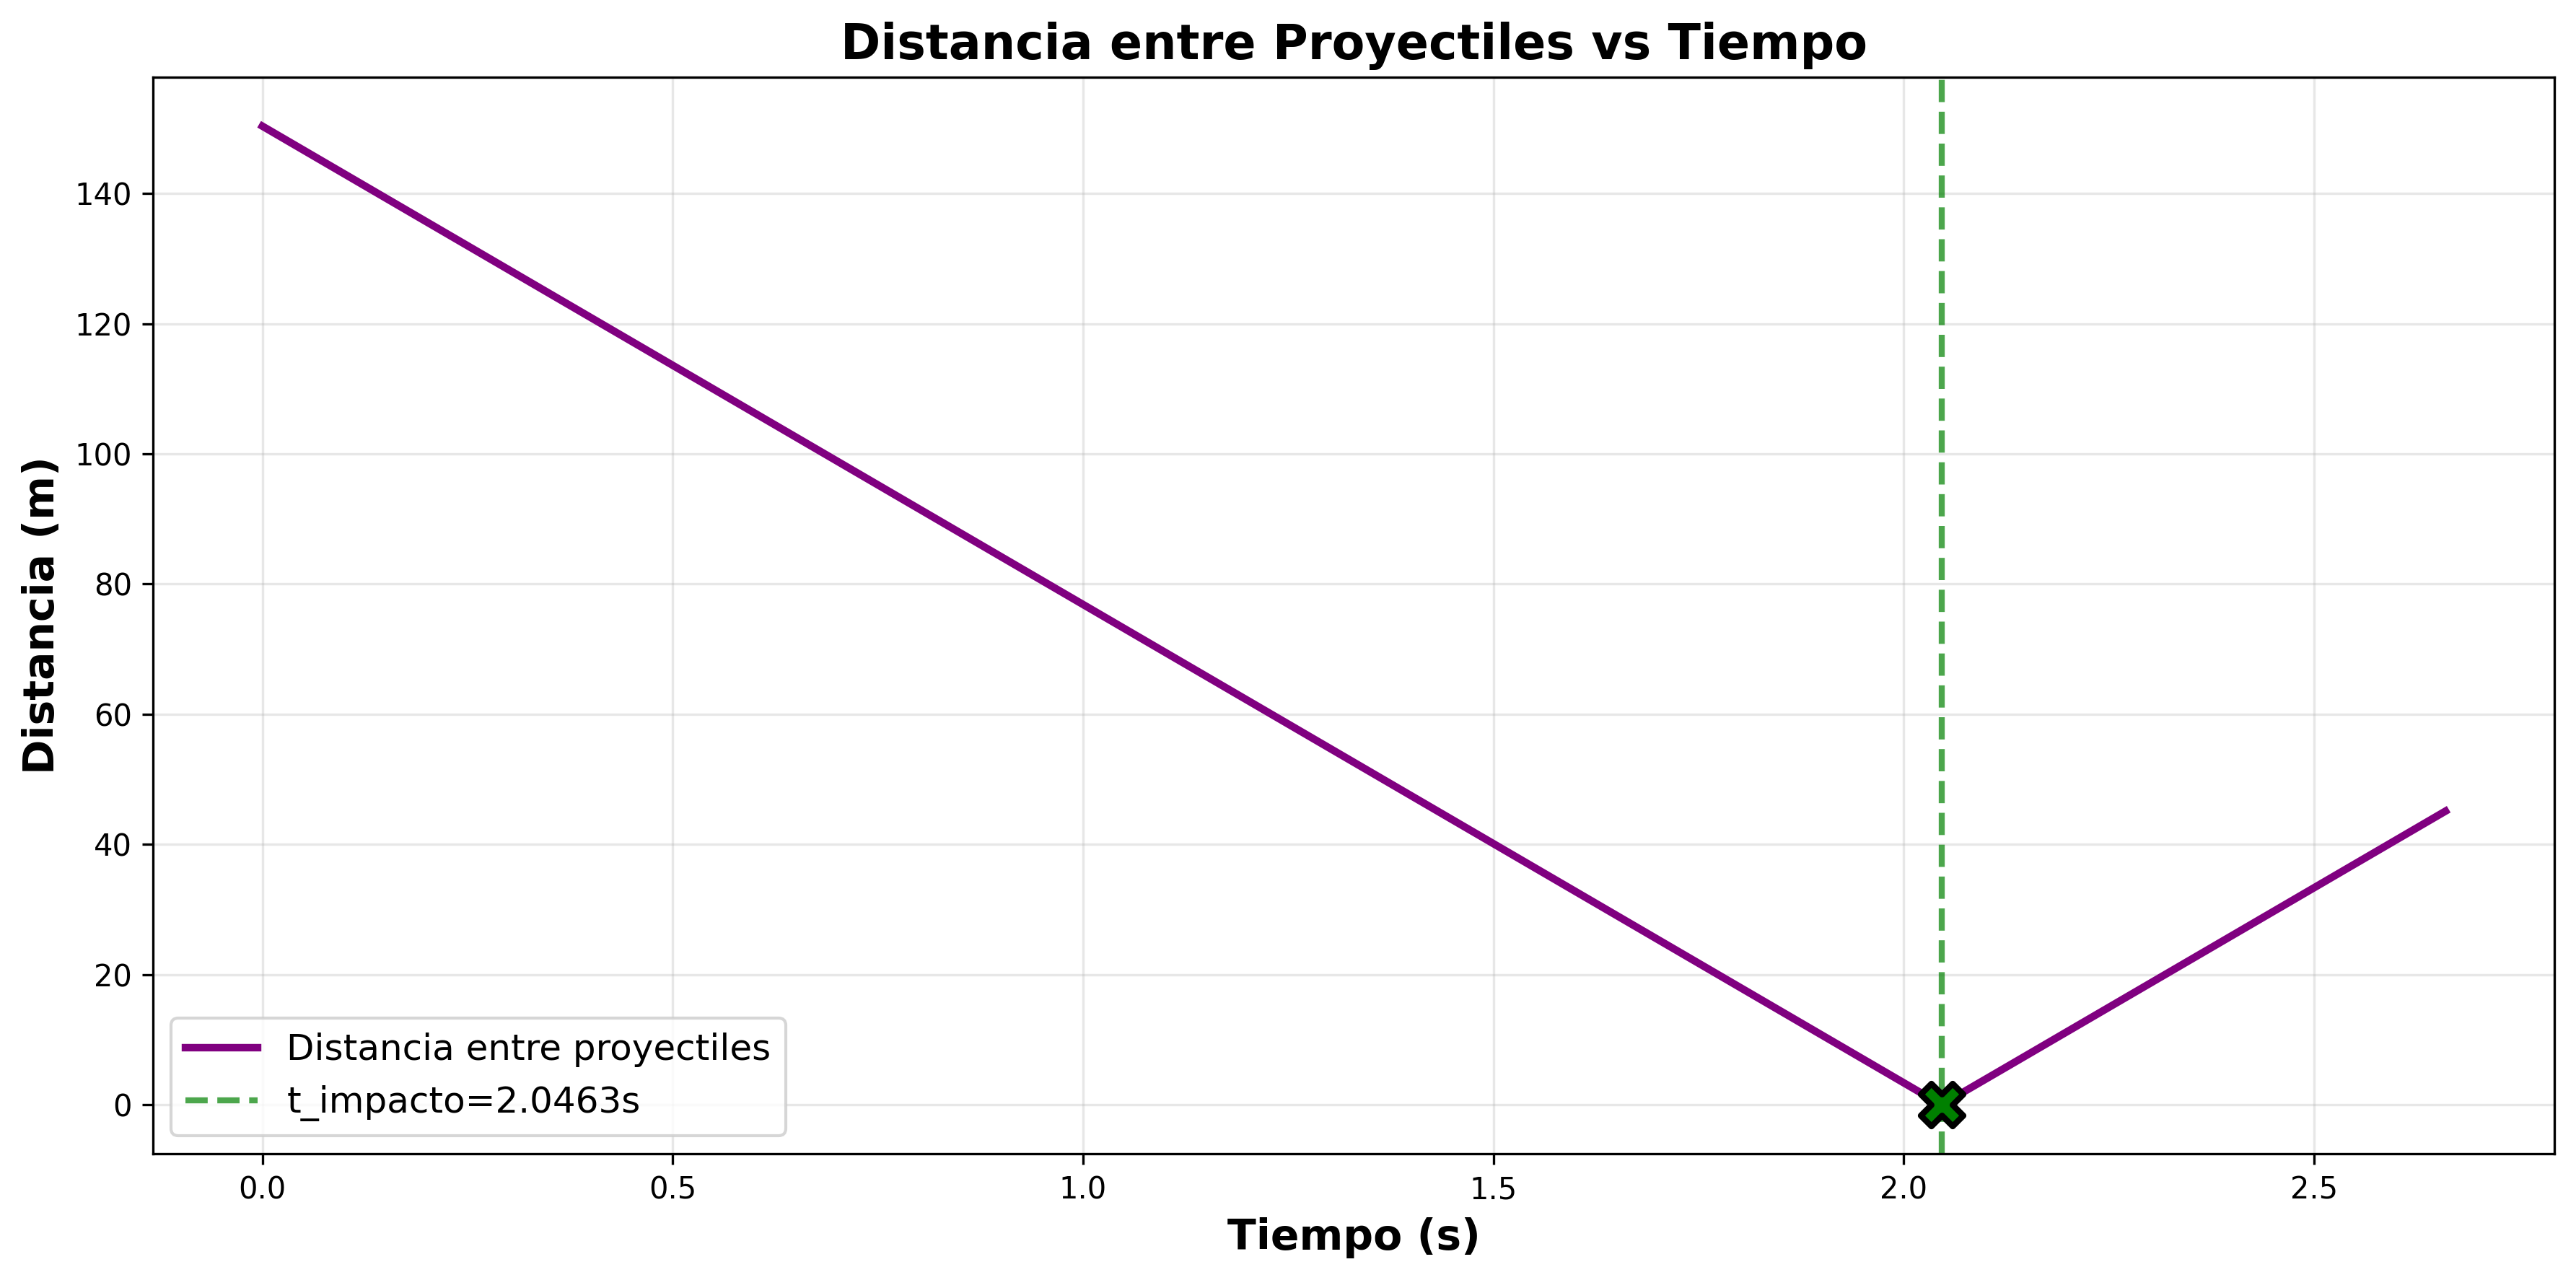
\includegraphics[width=\linewidth]{problema_3_distancia.png}
	\caption{Distancia entre los proyectiles en funci\'on del tiempo. El m\'inimo corresponde al punto de colisi\'on.}
	\label{fig:p3_dist}
\end{figure}

\begin{figure*}[ht]\centering
	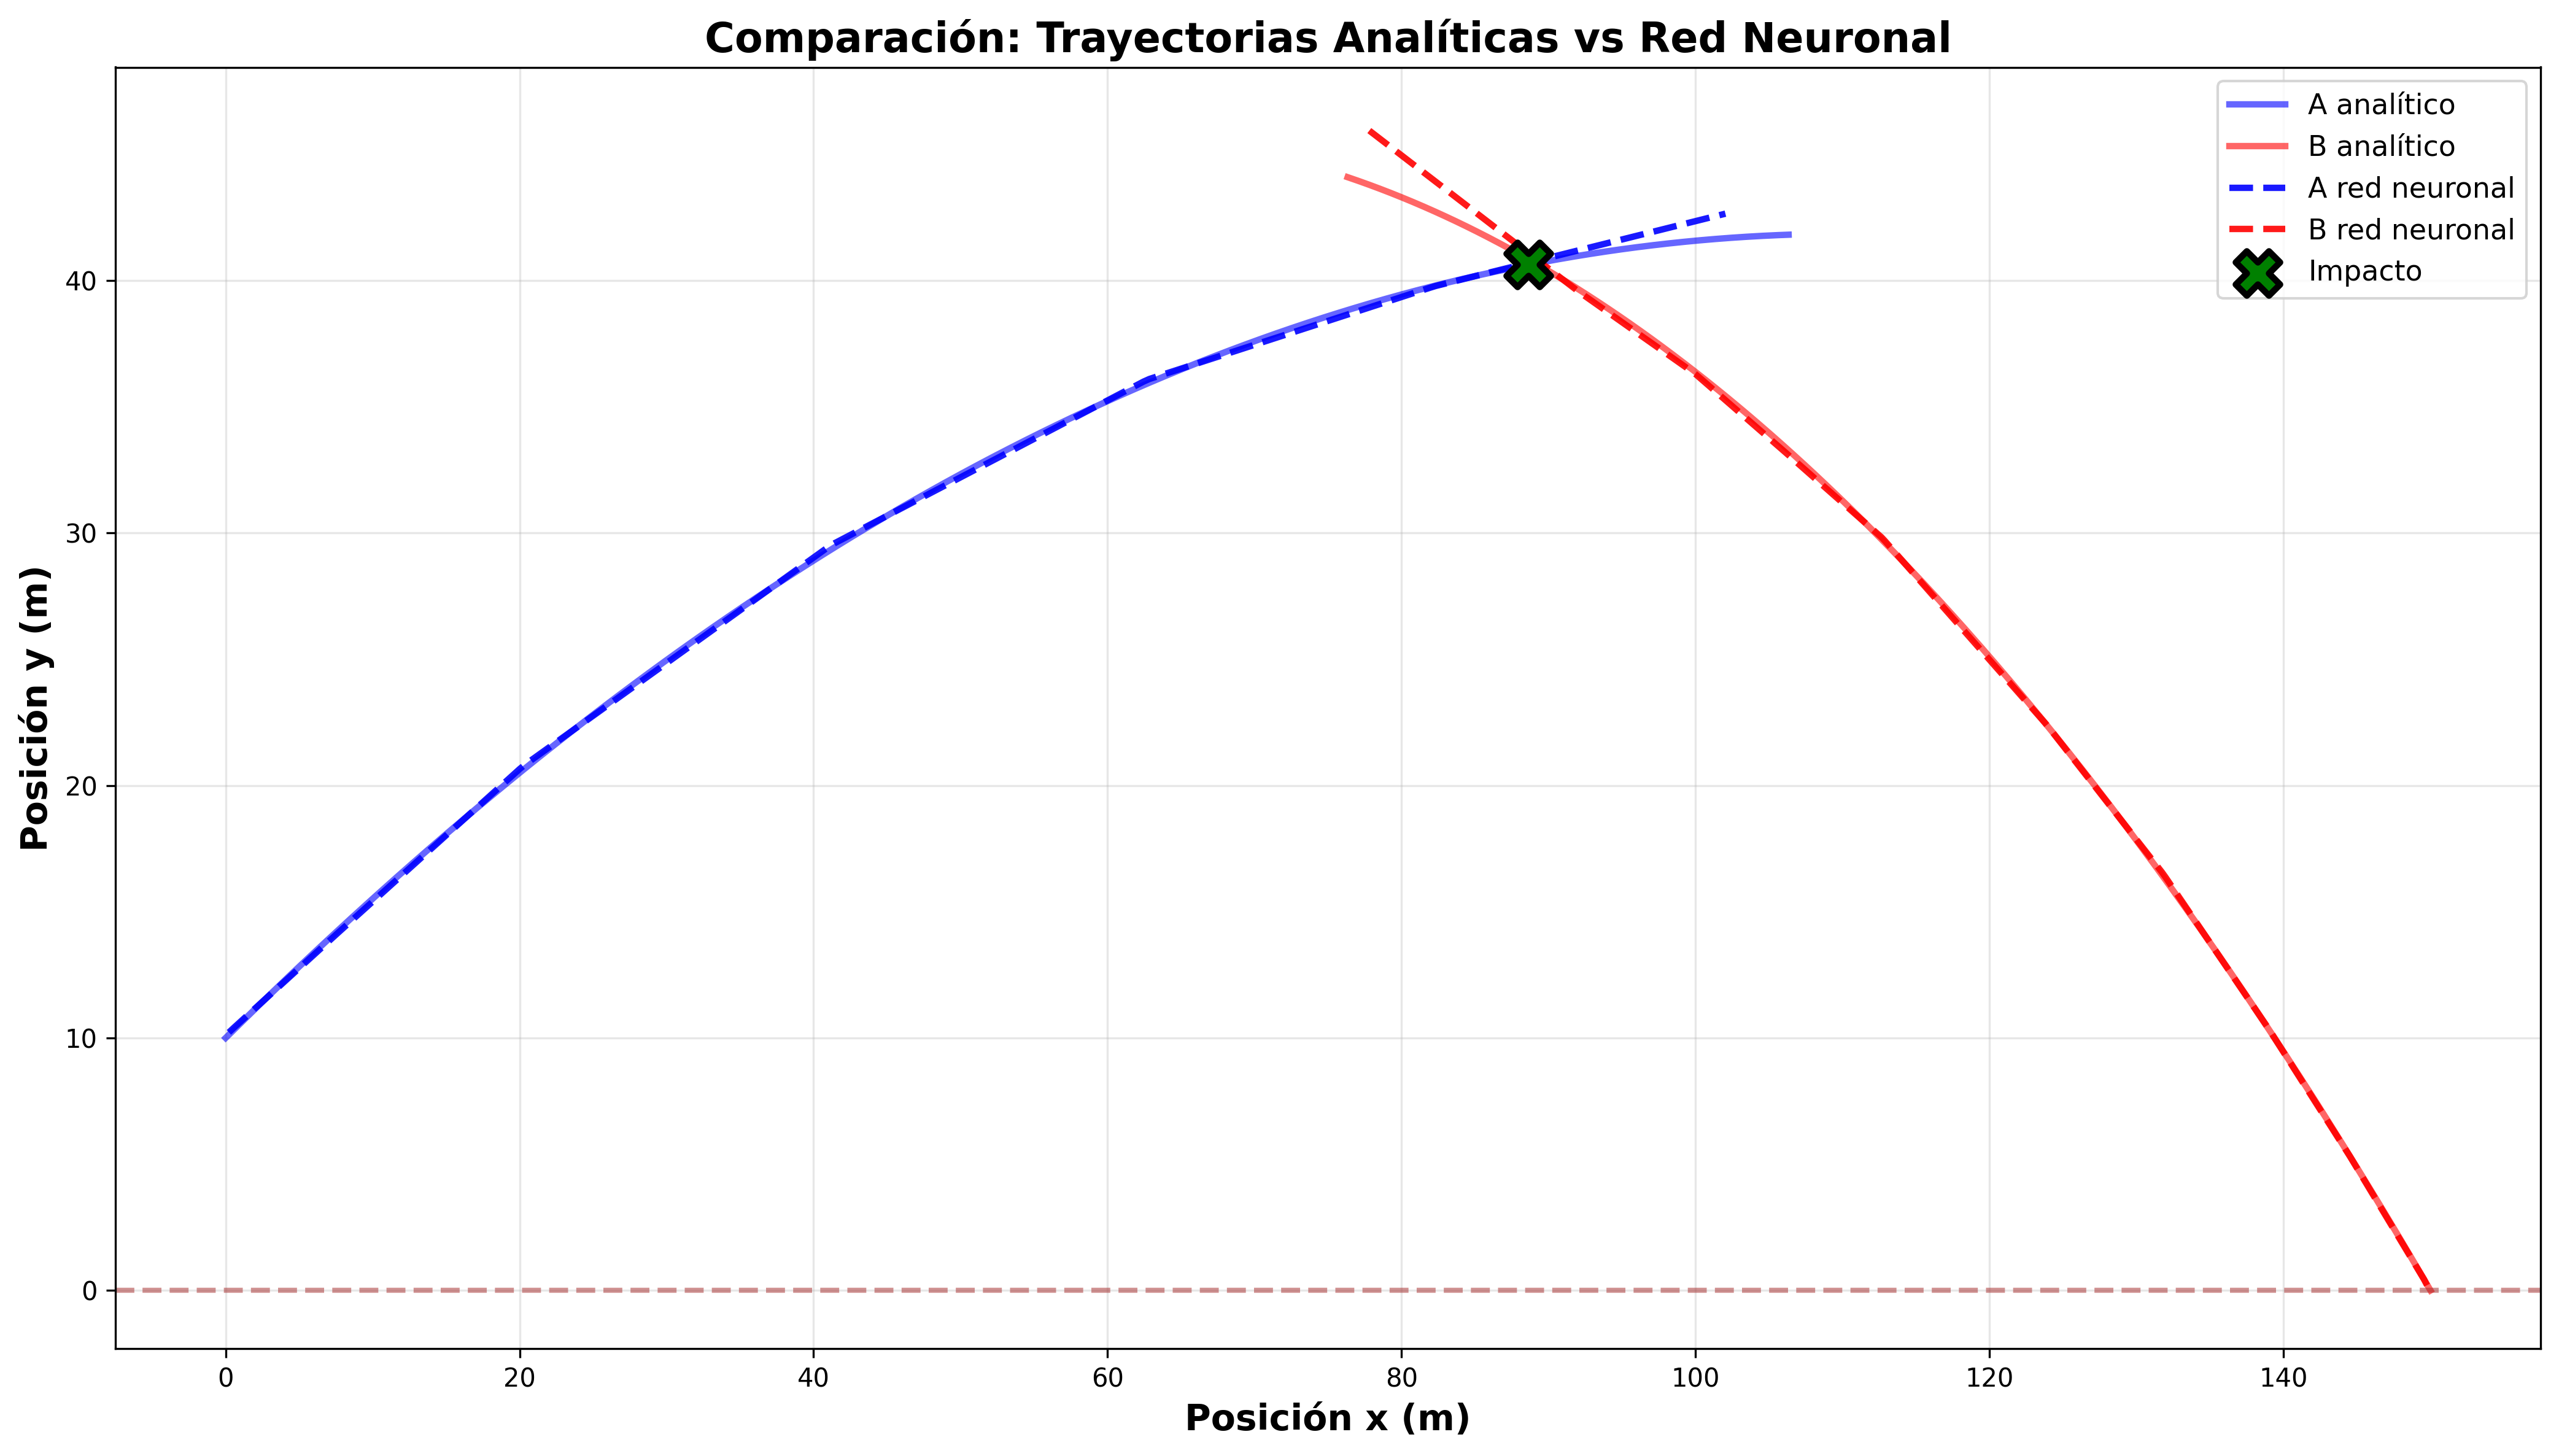
\includegraphics[width=\linewidth]{problema_3_nn_vs_analitico.png}
	\caption{Comparaci\'on entre las trayectorias anal\'iticas (s\'olidas) y las aproximaciones de las redes neuronales (punteadas).}
	\label{fig:p3_nn}
\end{figure*}

\begin{figure}[H]\centering
	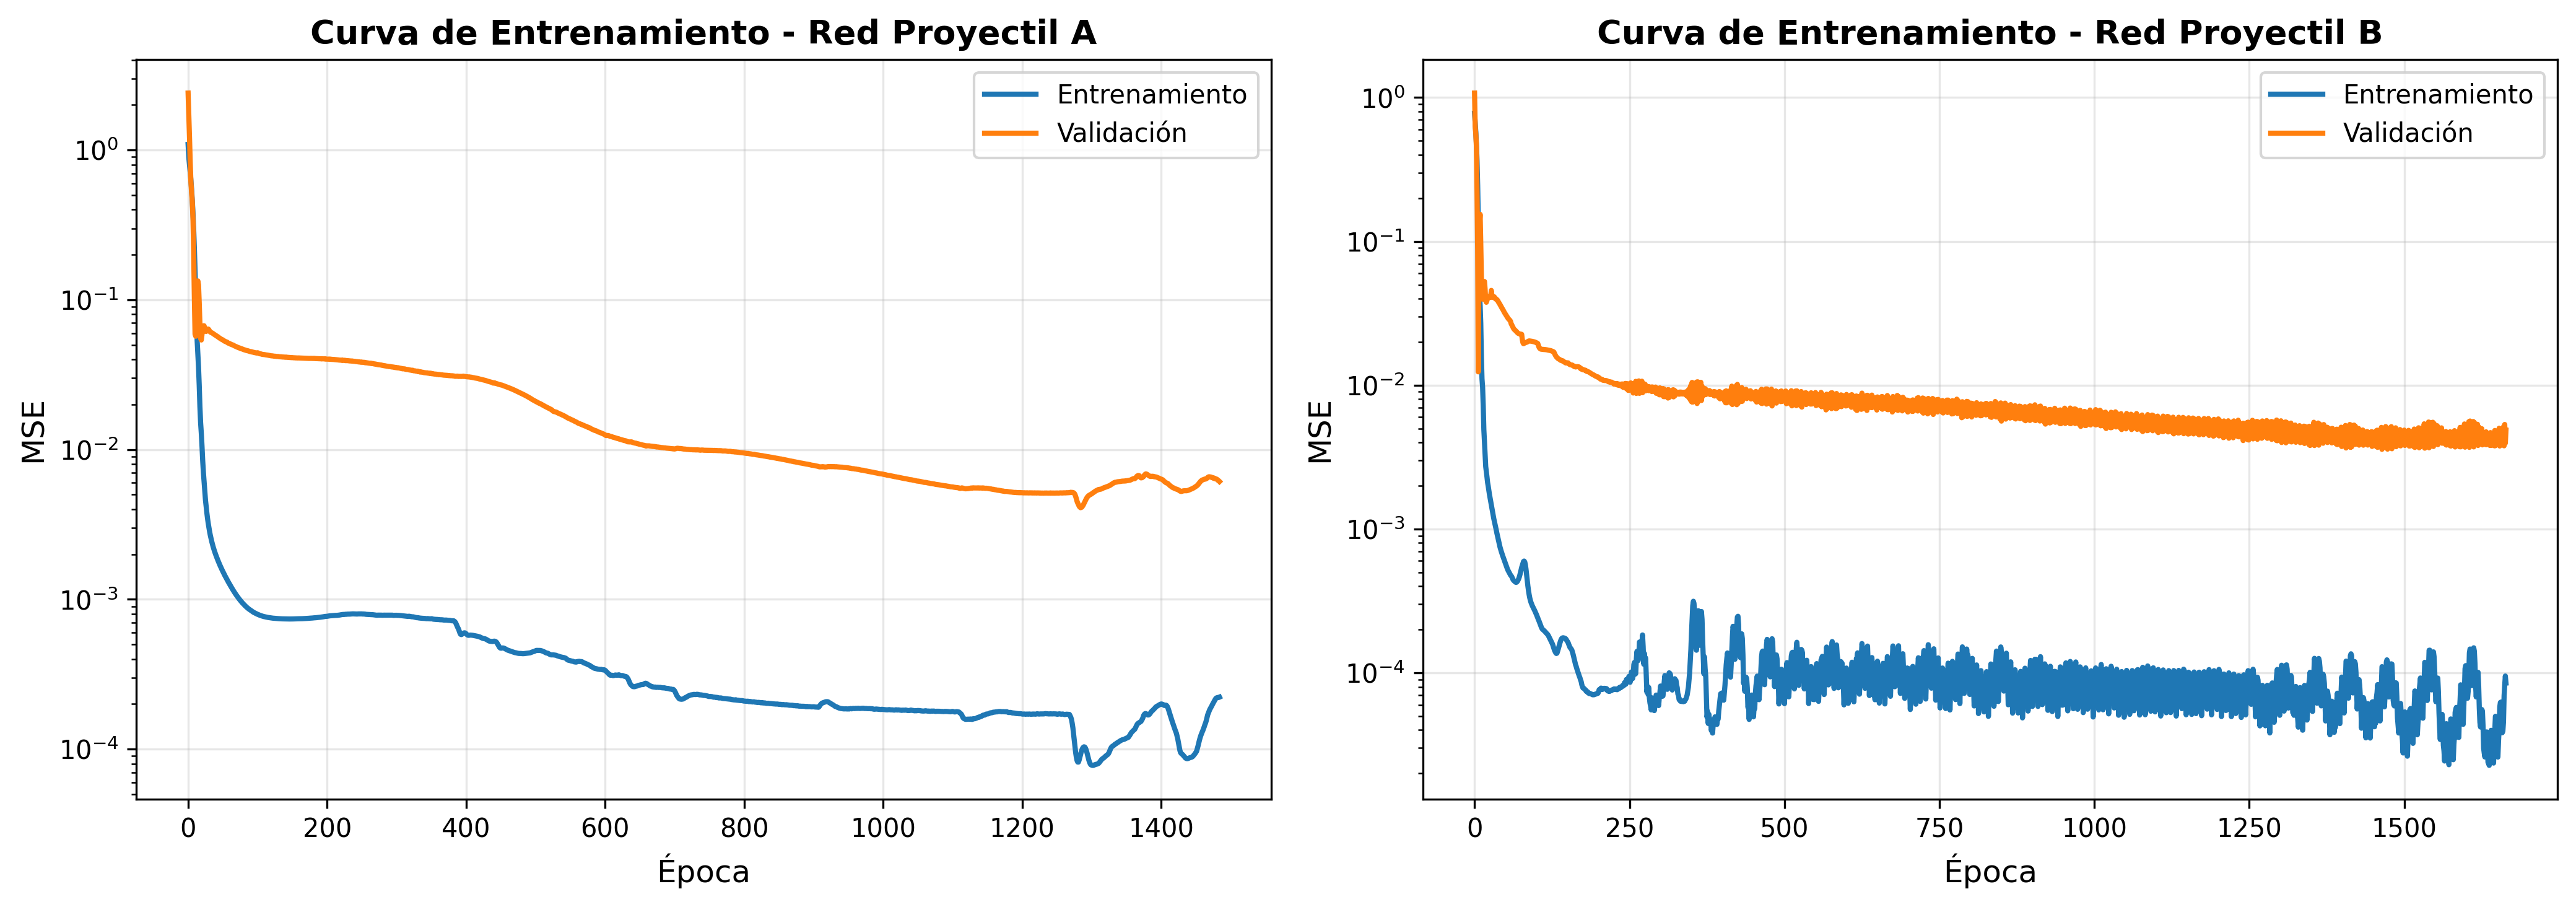
\includegraphics[width=\linewidth]{problema_3_loss.png}
	\caption{Curvas de entrenamiento para las redes neuronales de los proyectiles A y B.}
	\label{fig:p3_loss}
\end{figure}

%----------------------------------------------------------------------------------------

\section{Problema 4: Gemelo Digital de Sensor de Presi\'on (10 Puntos)}

Se construy\'o un gemelo digital de un sensor de presi\'on utilizando datos de no-linealidad (\%) en funci\'on de la presi\'on (Bar) \cite{gemelo2021}.

\subsection{Datos del Sensor}

\begin{table}[H]
	\caption{No-linealidad (\%) del sensor vs presi\'on (Bar)}
	\centering
	\begin{tabular}{cc}
		\toprule
		Presi\'on (Bar) & No-Linealidad (\%) \\
		\midrule
		0.0 & 0.00 \\
		0.1 & 0.01 \\
		0.2 & $-$0.02 \\
		0.3 & $-$0.01 \\
		0.4 & 0.02 \\
		0.5 & 0.05 \\
		0.6 & 0.09 \\
		0.7 & 0.12 \\
		0.8 & 0.06 \\
		0.9 & $-$0.05 \\
		1.0 & 0.00 \\
		\bottomrule
	\end{tabular}
	\label{tab:sensor}
\end{table}

\subsection{Arquitectura de la Red}

\begin{itemize}[noitemsep]
	\item Capa de entrada: 1 neurona (presi\'on normalizada)
	\item Capa oculta 1: 20 neuronas, activaci\'on $\tanh$
	\item Capa oculta 2: 20 neuronas, activaci\'on $\tanh$
	\item Capa de salida: 1 neurona, activaci\'on lineal
\end{itemize}

Se utiliz\'o Adam (lr=0.01), MSE, 3000 \'epocas con batch\_size de 11.

\subsection{Resultados}

\begin{figure}[H]\centering
	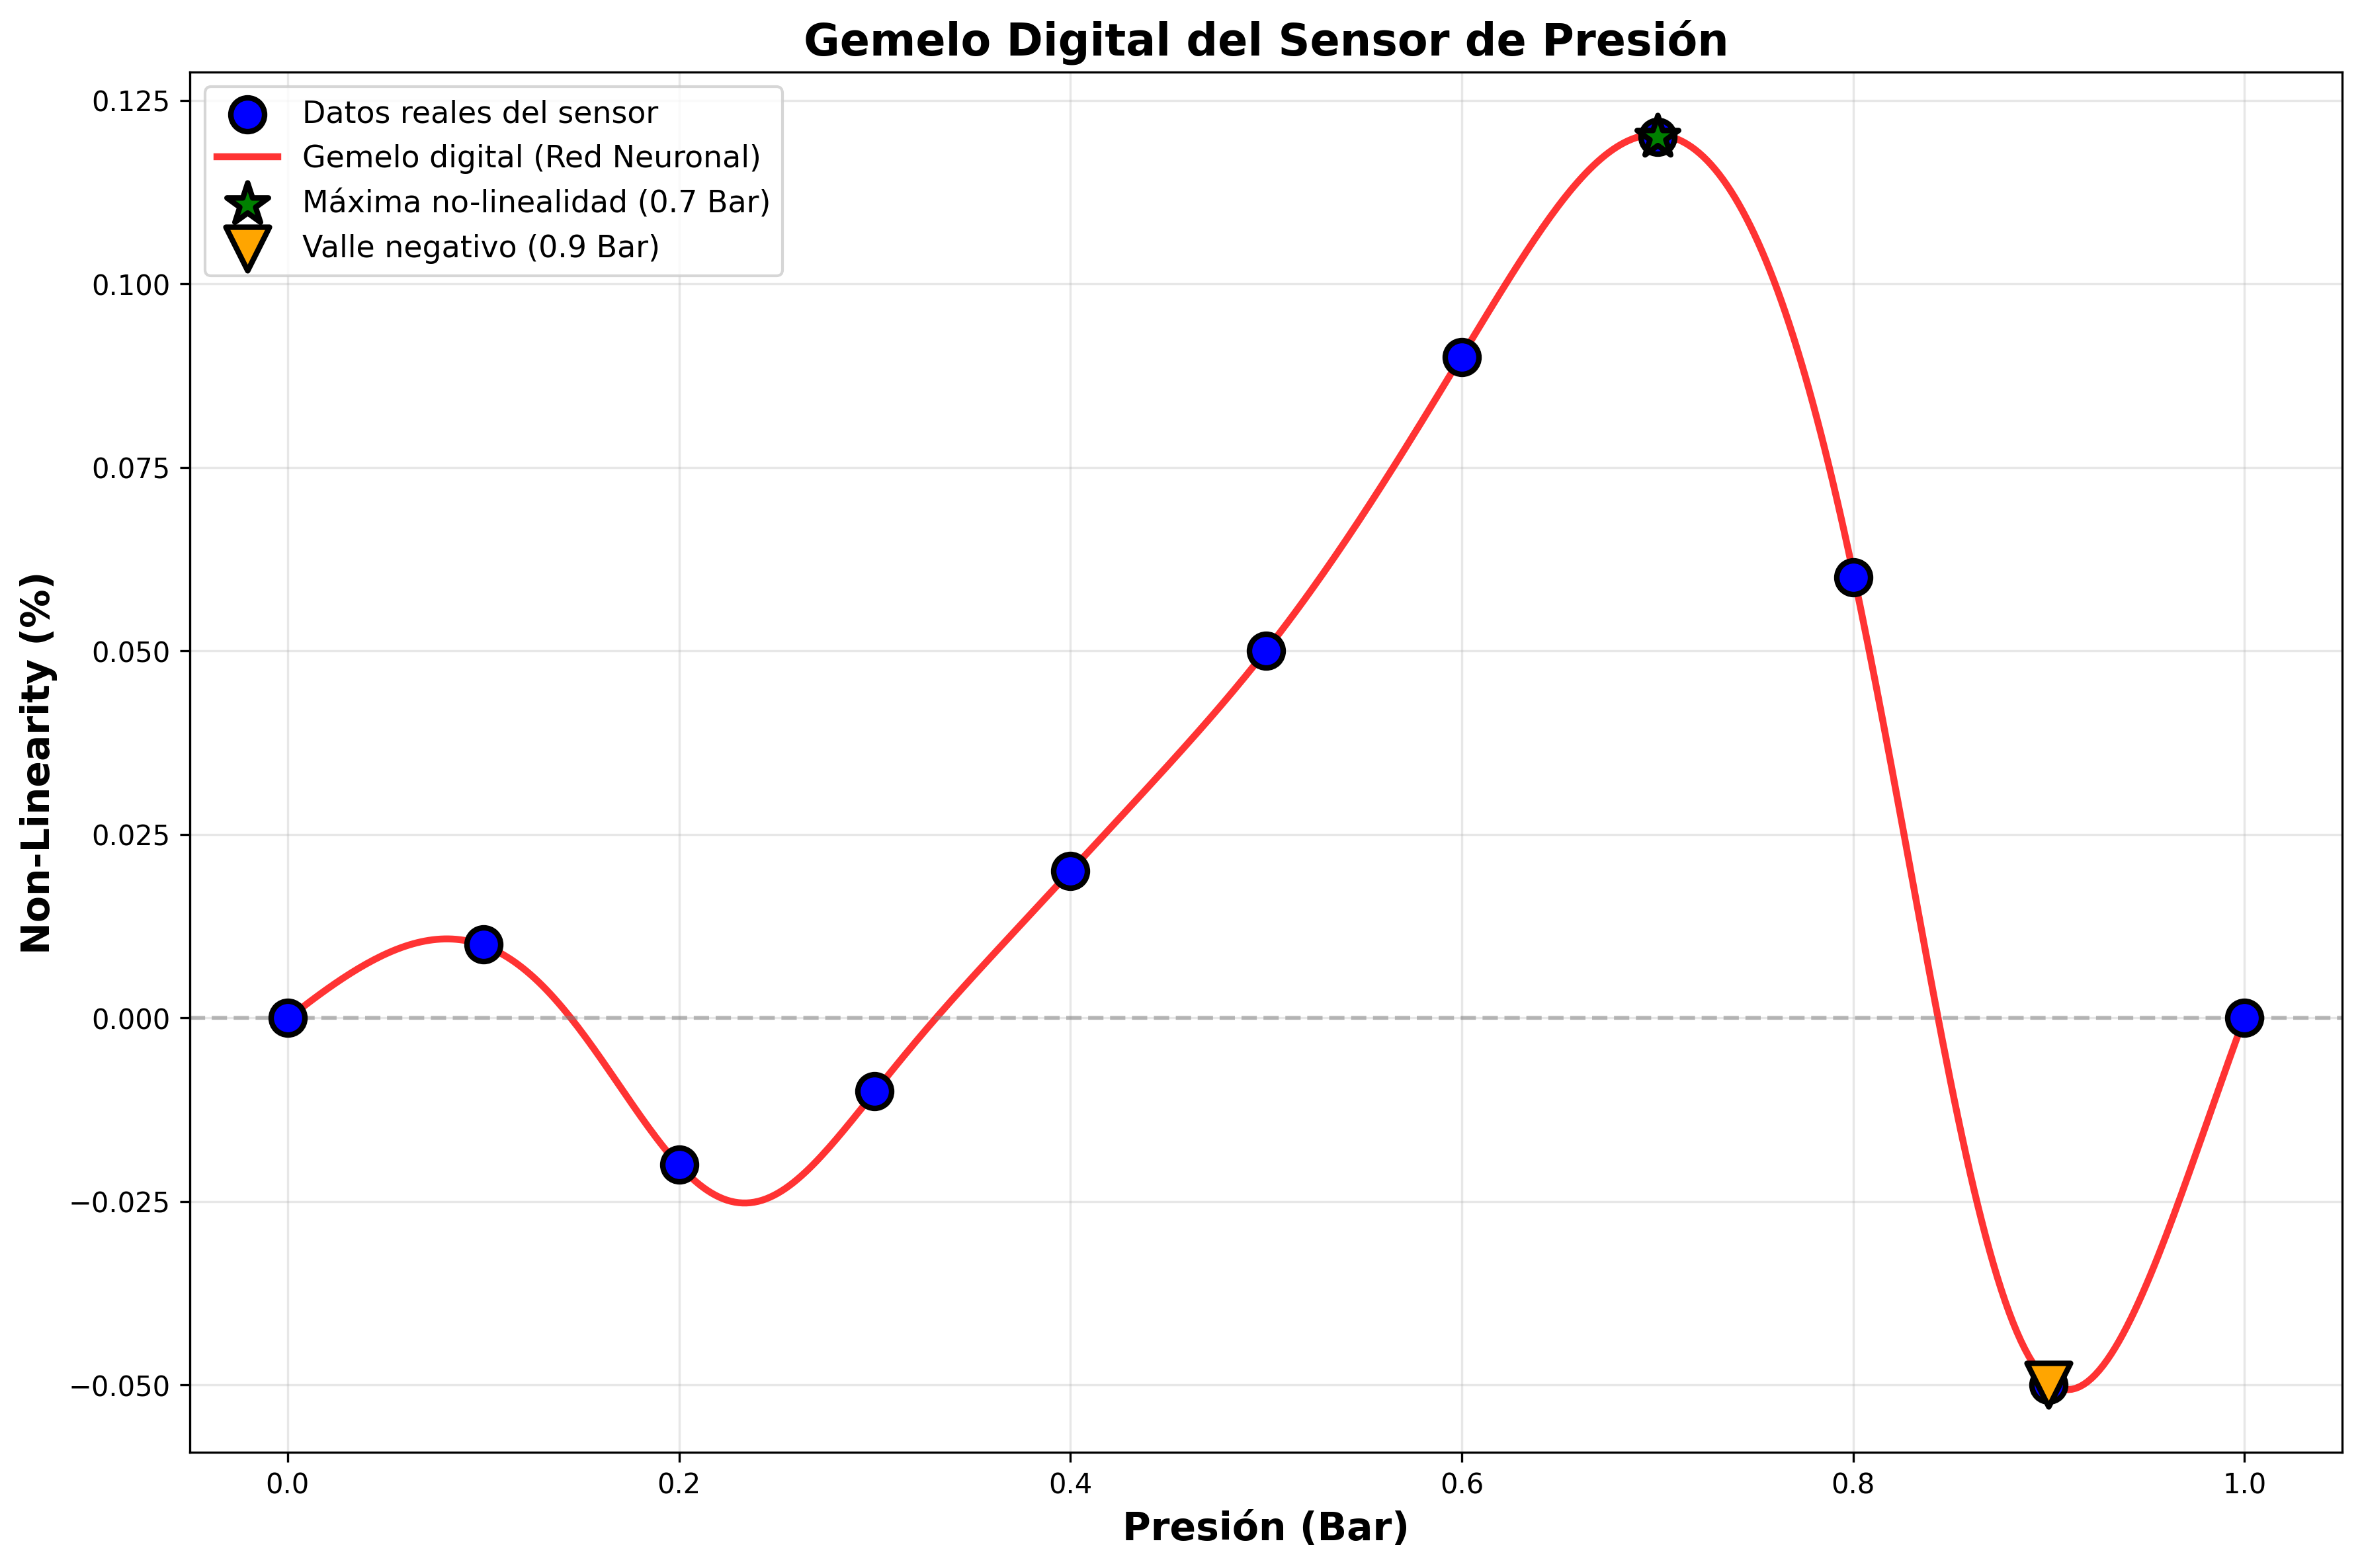
\includegraphics[width=\linewidth]{problema_4_gemelo_digital.png}
	\caption{Gemelo digital del sensor de presi\'on. Se destacan la m\'axima no-linealidad (0.7 Bar) y el valle negativo (0.9 Bar).}
	\label{fig:p4_gemelo}
\end{figure}

\begin{figure}[H]\centering
	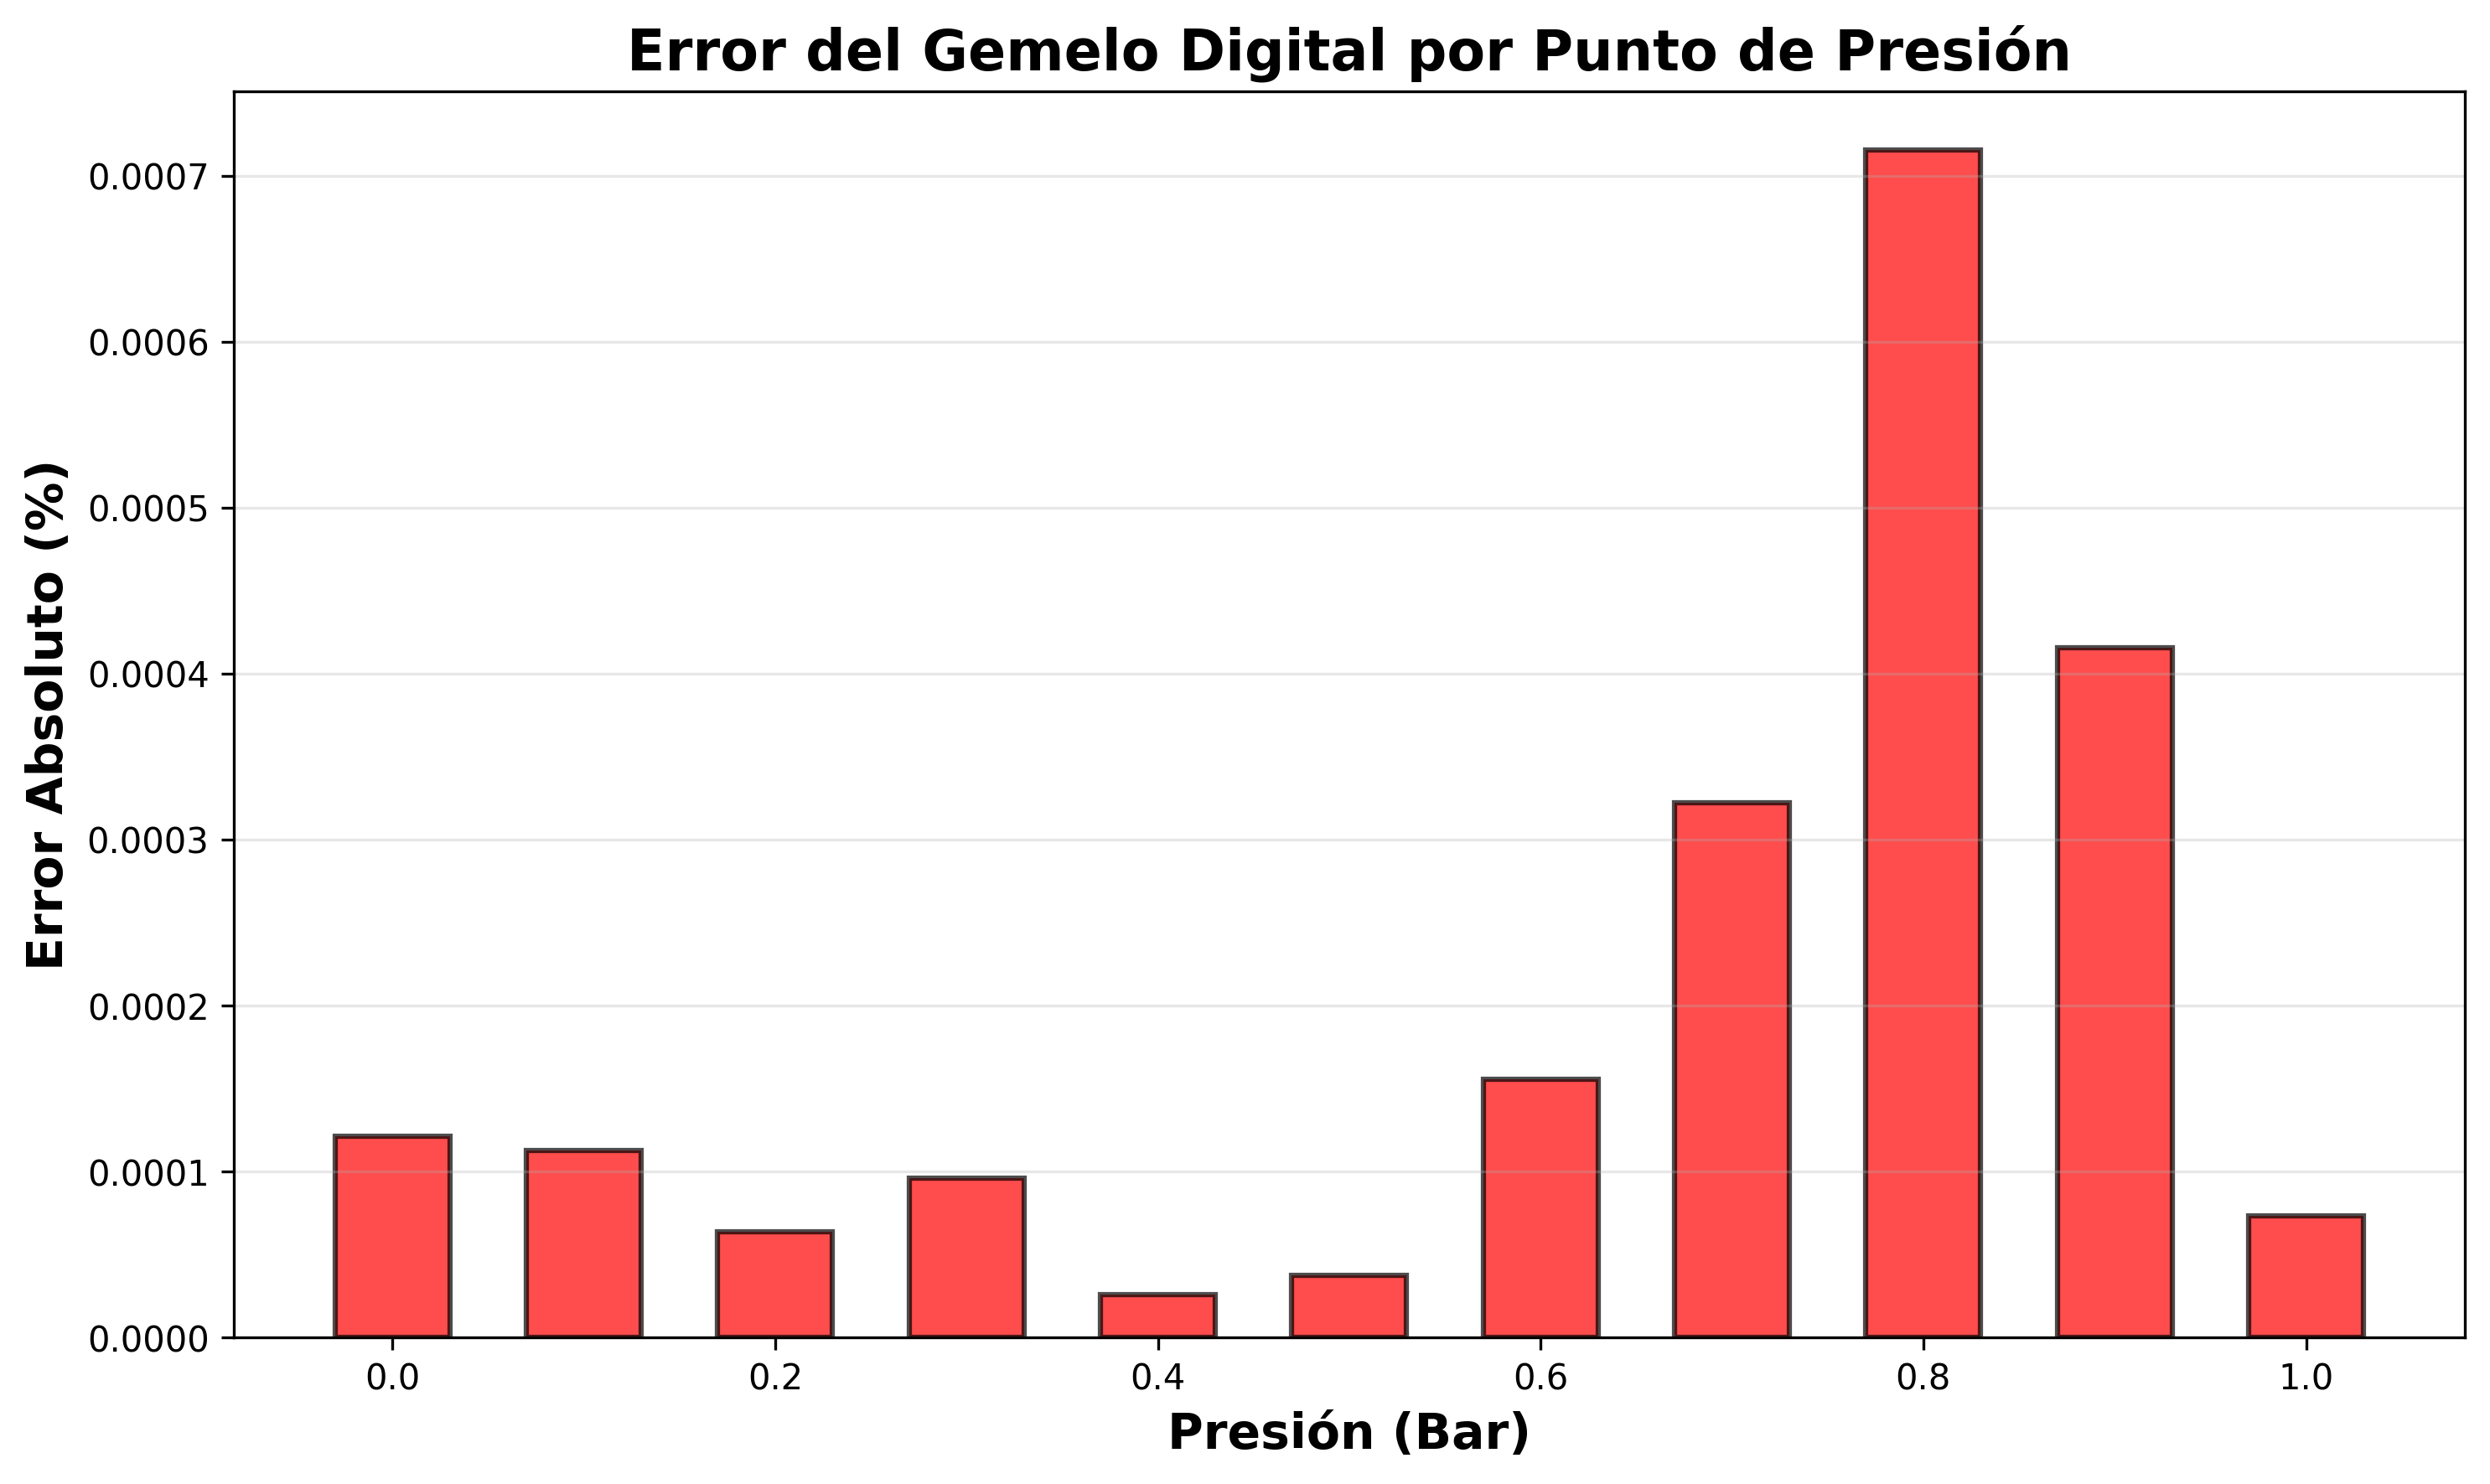
\includegraphics[width=\linewidth]{problema_4_error_barras.png}
	\caption{Error absoluto del gemelo digital por punto de presi\'on.}
	\label{fig:p4_error}
\end{figure}

\begin{figure}[H]\centering
	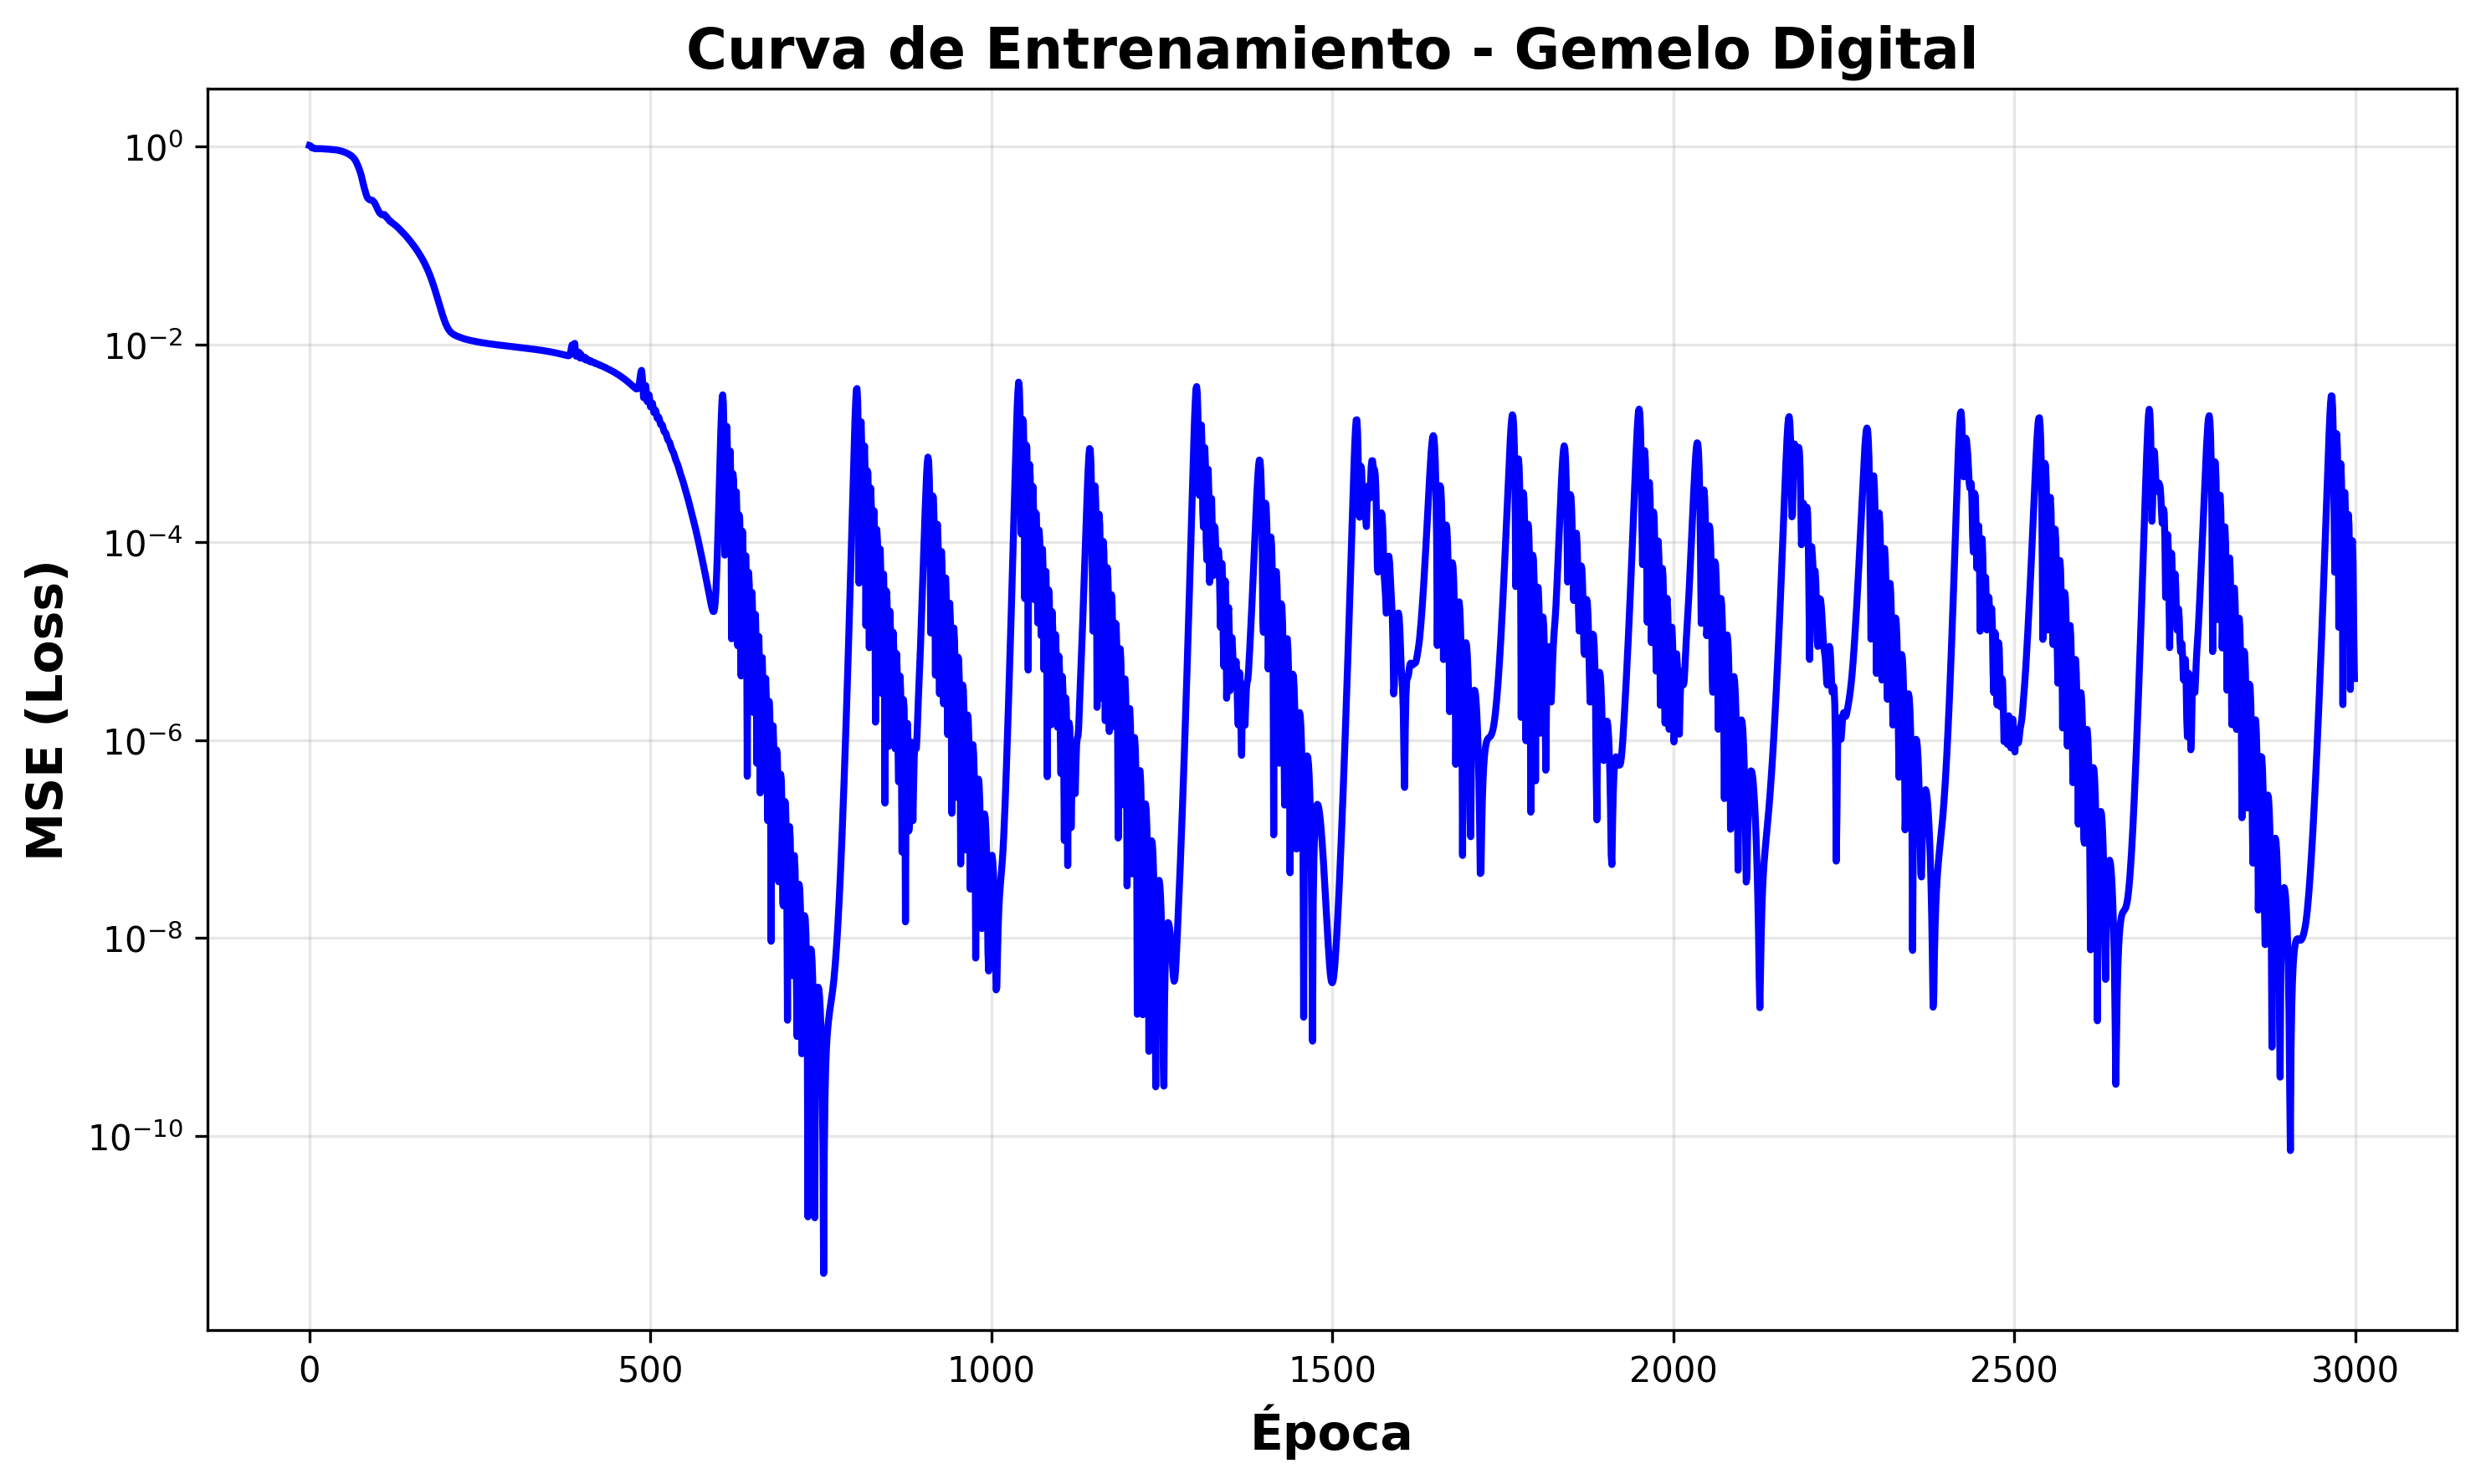
\includegraphics[width=\linewidth]{problema_4_loss.png}
	\caption{Curva de entrenamiento del gemelo digital.}
	\label{fig:p4_loss}
\end{figure}

\begin{figure}[H]\centering
	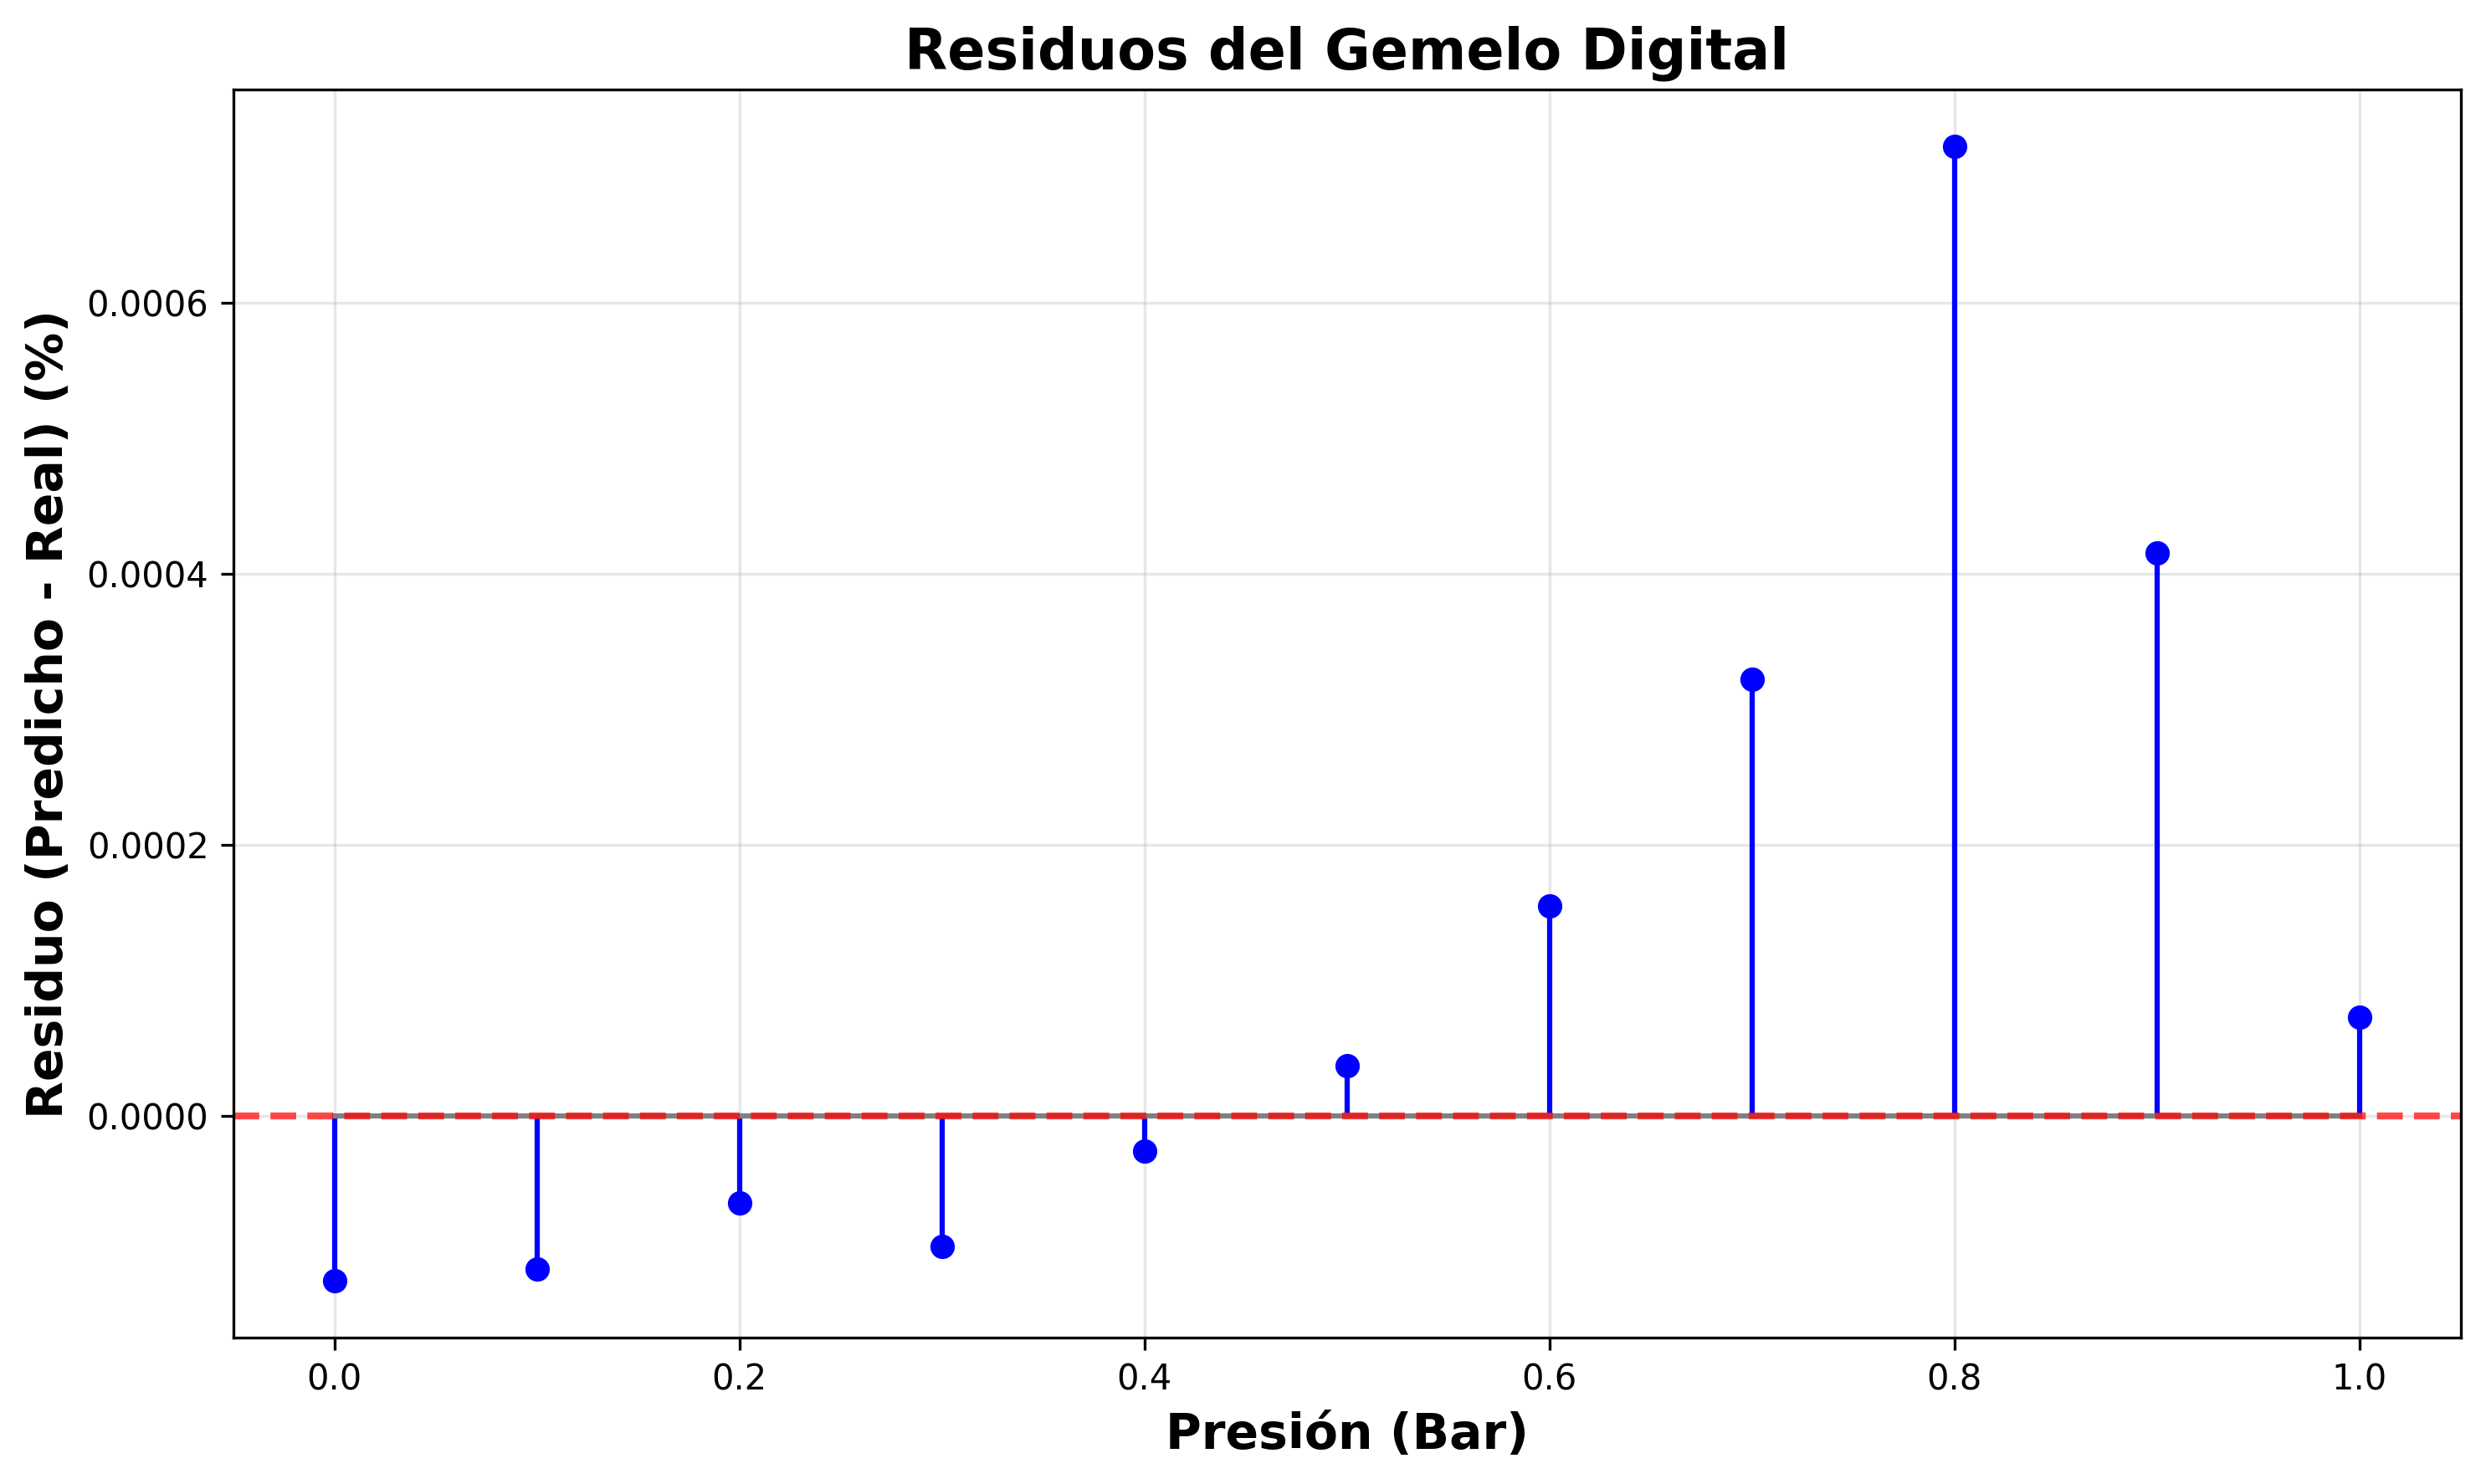
\includegraphics[width=\linewidth]{problema_4_residuos.png}
	\caption{Residuos (predicho $-$ real) del gemelo digital.}
	\label{fig:p4_residuos}
\end{figure}

%----------------------------------------------------------------------------------------

\section*{Conclusi\'on}
\addcontentsline{toc}{section}{Conclusi\'on}

En este examen parcial se demostr\'o la versatilidad de las redes neuronales tipo MLP para resolver diversos problemas de ingenier\'ia. En el Problema~1, las redes capturaron exitosamente las curvas de descarga de bater\'ia a cuatro temperaturas distintas. En el Problema~2, se lograron aproximar seis pares de curvas polinomiales y localizar con precisi\'on sus puntos de intersecci\'on. El Problema~3 mostr\'o c\'omo las redes neuronales pueden complementar soluciones anal\'iticas en problemas de cinem\'atica de proyectiles. Finalmente, el Problema~4 valid\'o el concepto de gemelo digital aplicado a sensores de presi\'on, reproduciendo fielmente el comportamiento de no-linealidad del sensor.

Los resultados confirman que, con una arquitectura adecuada y un proceso de entrenamiento bien configurado, las redes neuronales artificiales constituyen una herramienta eficaz para el modelado y la aproximaci\'on de sistemas f\'isicos e ingenieriles.

%----------------------------------------------------------------------------------------

\phantomsection
\bibliographystyle{unsrt}
\bibliography{sample}

%----------------------------------------------------------------------------------------

\end{document}
